%% 
%% Copyright 2019-2024 Elsevier Ltd
%% 
%% This file is part of the 'CAS Bundle'.
%% --------------------------------------
%% 
%% It may be distributed under the conditions of the LaTeX Project Public
%% License, either version 1.3c of this license or (at your option) any
%% later version.  The latest version of this license is in
%%    http://www.latex-project.org/lppl.txt
%% and version 1.3c or later is part of all distributions of LaTeX
%% version 1999/12/01 or later.
%% 
%% The list of all files belonging to the 'CAS Bundle' is
%% given in the file `manifest.txt'.
%% 
%% Template article for cas-sc documentclass for 
%% double column output.

\documentclass[a4paper,fleqn]{cas-sc}

% If the frontmatter runs over more than one page
% use the longmktitle option.

%\documentclass[a4paper,fleqn,longmktitle]{cas-sc}
\usepackage{amssymb}
\usepackage{amsthm}
\newtheorem{proposition}{Proposition}[section]
\newtheorem{remark}{Remark}[section]
\usepackage{caption}

\captionsetup[table]{
	labelsep=period,
	singlelinecheck=false
}
\usepackage{graphicx}
\usepackage{algorithm}
\usepackage{algpseudocode}
\renewcommand{\algorithmicrequire}{\textbf{Input:}}
\renewcommand{\algorithmicensure}{\textbf{Output:}}
\usepackage{booktabs}
\usepackage{tabularx}
\usepackage{array}
\usepackage[section]{placeins}
\usepackage{float}
\usepackage{multirow}
\usepackage{siunitx}
\newcolumntype{Y}{>{\raggedright\arraybackslash}X}
%\usepackage[numbers]{natbib}
\usepackage[authoryear]{natbib}
%\usepackage[authoryear,longnamesfirst]{natbib}
%\usepackage{hyperref}
\usepackage{xcolor}
% Reduce spacing around figures and tables
\setlength{\textfloatsep}{10pt plus 2pt minus 2pt}
\setlength{\intextsep}{8pt plus 2pt minus 2pt}
\setlength{\floatsep}{8pt plus 2pt minus 2pt}
\setlength{\abovecaptionskip}{4pt}
\setlength{\belowcaptionskip}{2pt}
\definecolor{journalblue}{RGB}{0,102,170}

\hypersetup{
    colorlinks=true,
    linkcolor=blue,
    citecolor=journalblue,
    urlcolor=journalblue
}
% Anonymous manuscript: suppress the template's otherwise empty ORCID line.
\RenewDocumentCommand{\printorcid}{}{}
% Anonymous manuscript: remove the empty short-author field and its orphan colon
% from the CAS first-page footer.
\ExplSyntaxOn
\cs_set:Npn \__first_footerline:
  { \group_begin: \small \rmfamily \itshape Preprint~submitted~to~Elsevier \group_end: }
\ExplSyntaxOff
%%%Author macros
\def\tsc#1{\csdef{#1}{\textsc{\lowercase{#1}}\xspace}}
\tsc{WGM}
\tsc{QE}
%%%

% Uncomment and use as if needed
%\newtheorem{theorem}{Theorem}
%\newtheorem{lemma}[theorem]{Lemma}
%\newdefinition{rmk}{Remark}
%\newproof{pf}{Proof}
%\newproof{pot}{Proof of Theorem \ref{thm}}

\begin{document}
\let\WriteBookmarks\relax
\def\floatpagepagefraction{1}
\def\textpagefraction{.001}

% Short title
\shorttitle{}    

% Short author
\shortauthors{}  

% Main title of the paper
\title [mode = title]{RAPTOR: Resource-Aware Physics-Token Operator with Residual Local Adaptation for Aerodynamic Field Reconstruction}  



%% First author
%%
%% Options: Use if required
%% eg: \author[1,3]{Author Name}[type=editor,
%%       style=chinese,
%%       auid=000,
%%       bioid=1,
%%       prefix=Sir,
%%       orcid=0000-0000-0000-0000,
%%       facebook=<facebook id>,
%%       twitter=<twitter id>,
%%       linkedin=<linkedin id>,
%%       gplus=<gplus id>]
%
%\author[1]{Xu Cheng}%[<options>]
%
%% Corresponding author indication
%\cormark[1]
%
%% Footnote of the first author
%\fnmark[1]
%
%% Email id of the first author
%\ead{xucheng0117@njust.edu.cn}
%
%% URL of the first author
%\ead[url]{orcid=https://orcid.org/0009-0008-1936-1021}
%
%% Credit authorship
%% eg: \credit{Conceptualization of this study, Methodology, Software}
%
%\credit{Conceptualization, Methodology, Visualization, Writing -- original draft}
%
%% Address/affiliation
%\affiliation[1]{organization={School of Mathematics and Statistics Nanjing University of Science and Technology},
%%            addressline={}, 
%            city={Nanjing},
%%          citysep={}, % Uncomment if no comma needed between city and postcode
%            postcode={210094}, 
%            state={Jiangsu},
%            country={P. R. China}}
%
%\author[2]{}%[]
%
%% Footnote of the second author
%\fnmark[2]
%
%% Email id of the second author
%\ead{}
%
%% URL of the second author
%\ead[url]{}
%
%% Credit authorship
%\credit{}
%
%% Address/affiliation
%\affiliation[2]{organization={},
%            addressline={}, 
%            city={},
%%          citysep={}, % Uncomment if no comma needed between city and postcode
%            postcode={}, 
%            state={},
%            country={}}
%
%% Corresponding author text
%\cortext[1]{Corresponding author}
%
%% Footnote text
%\fntext[1]{}

% For a title note without a number/mark
%\nonumnote{}

% Here goes the abstract

\begin{abstract}
	Aerodynamic field reconstruction on unstructured discretizations requires long-range communication while preserving local geometric detail, yet dense node-level attention incurs quadratic computational and memory cost. We propose RAPTOR, a resource-aware physics-token operator that augments slice-based Physics-Attention with a sparse $K$-nearest-neighbor residual adapter. The token branch captures global interactions, while the adapter restores neighborhood-scale information directly in node space. A zero-initialized bounded gate makes each block identical to its Physics-Attention backbone at initialization and progressively activates the local correction. For a fixed input state, each head's frozen node-mixing matrix has rank at most the number of slices $S$. With precomputed neighborhoods, RAPTOR retains $\mathcal{O}(NS+S^2+NK)$ connectivity without constructing dense $N\times N$ attention. We evaluate Reynolds-number and angle-of-attack extrapolation on AirfRANS and automobile and aircraft surface-pressure-coefficient reconstruction on Mixed-3D. Under fixed splits and one training seed, RAPTOR attains the lowest macro relative $L_2$ error among the evaluated models on both AirfRANS tasks. Relative to Transolver-Tiny, it reduces the macro relative $L_2$ error by $2.68\%$ on Reynolds-number extrapolation and $5.37\%$ on angle-of-attack extrapolation. On Mixed-3D, it reduces standardized-space MSE by $6.77\%$ for automobiles and $8.57\%$ for aircraft. All accuracy experiments use $N=4096$ on one RTX~4050 Laptop GPU. In a separate node-scaling profile, RAPTOR completes a mixed-precision training step at $N=16384$ in $66.99$\,ms with $410.31$\,MiB peak allocated memory, whereas dense attention is not run beyond $N=8192$ to avoid memory oversubscription. These results support resource-efficient aerodynamic reconstruction with favorable precomputed-graph scaling over the tested range.
\end{abstract}


% Use if graphical abstract is present
%\begin{graphicalabstract}
%\includegraphics{}
%\end{graphicalabstract}

% Research highlights

% Keywords
% Each keyword is seperated by \sep
\begin{keywords}
Aerodynamic field reconstruction \sep
Physics-token neural operator \sep
Sparse local adaptation \sep
Computational scalability \sep
Unstructured discretizations
\end{keywords}

\maketitle

% Main text
\section{Introduction}
\label{sec:introduction}

High-fidelity computational fluid dynamics (CFD) is an essential tool for aerodynamic analysis and engineering design. Accurately solving the governing equations is often computationally expensive, particularly when repeated simulations are required for complex aerodynamic configurations such as airfoils, automobiles, and aircraft. Data-driven surrogate models provide an alternative by learning direct mappings from geometry and flow conditions to the corresponding physical fields, thereby reducing the cost of repeated CFD simulations \citep{ref04,ref05}. Neural operators have emerged as an effective framework for learning mappings between function spaces \citep{ref07,ref08}. However, aerodynamic field reconstruction on complex unstructured geometries remains challenging because it requires simultaneous modeling of long-range physical dependencies and local features such as surface curvature, boundary layers, leading-edge gradients, and wakes.

Existing architectures address these requirements from different perspectives. Point-cloud models such as PointNet aggregate global information through shared point encoders and symmetric pooling \citep{ref11}, whereas graph neural networks propagate node features through mesh edges or local neighborhood connections \citep{ref12,ref14}. These architectures introduce useful geometric inductive biases, but models relying exclusively on local propagation generally require multiple layers to establish cross-region communication. Global self-attention directly models non-local dependencies. However, applying dense attention to $N$ nodes requires an $N\times N$ interaction matrix. For three-dimensional surface discretizations containing thousands or more nodes, this quadratic growth limits practical scalability.

Latent-token and physics-token operators reduce the cost of global interaction by projecting nodes into a compact latent space \citep{ref19,ref20,ref23}. Physics-Attention, in particular, softly assigns nodes to a limited number of physical slices, performs attention in the slice space, and maps the updated representations back to the original nodes \citep{ref20}. This mechanism enables efficient cross-region communication without dense node-level attention. But token compression may weaken local features associated with surface curvature, boundary layers, and high-gradient regions. A central challenge is therefore to recover such information without disrupting the global operator or reintroducing quadratic complexity. This challenge is especially relevant under limited hardware budgets, since the high-memory GPUs required for larger token sets, wider representations, and extensive hyperparameter searches are not universally accessible. Developing more effective interaction structures for consumer-grade GPUs is thus important for improving the accessibility and reproducibility of aerodynamic field reconstruction.

To address this limitation, we propose RAPTOR, a residual-augmented physics-token operator for aerodynamic field reconstruction. RAPTOR retains slice-based Physics-Attention as its global backbone and equips each operator block with a sparse \(K\)-nearest-neighbor (\(K\)-NN) geometric adapter. The global branch captures cross-region dependencies through compressed slice interactions, whereas the local branch operates directly in node space to recover neighborhood information weakened by token compression. A zero-initialized bounded gate preserves the backbone at initialization and permits the local residual to be learned progressively.
The main contributions of this work are summarized as follows:

\begin{enumerate}
	\item We propose RAPTOR, a resource-aware hybrid neural operator that couples token-mediated global interaction with an explicit sparse $K$-nearest-neighbor residual correction in node space. Unlike mechanisms that modify only token assignment, the proposed adapter introduces direct neighborhood-level dependencies alongside the compressed global pathway. Once the neighborhoods are available, each block retains
	$\mathcal{O}(NS+S^2+NK)$ connectivity complexity without constructing a dense $N\times N$ attention matrix.
	
	\item We introduce a zero-initialized bounded residual gate for integrating the local correction. At initialization, every RAPTOR block is exactly equivalent to its Physics-Attention backbone; during optimization, the gate progressively controls the contribution of the node-space adapter. We further characterize the token branch through its per-head conditional node-mixing rank under frozen, input-dependent assignments and attention weights, clarifying the representation bottleneck that motivates the complementary local pathway.
	
	\item We conduct a unified evaluation on two-dimensional AirfRANS extrapolation tasks and three-dimensional automobile and aircraft surface-pressure-coefficient reconstruction tasks from the Mixed-3D benchmark. Under the reported fixed splits and single-seed protocol, RAPTOR achieves the lowest macro relative $L_2$ error among the evaluated models on both AirfRANS tasks and reduces the standardized-space MSE of Transolver-Tiny by $6.77\%$ and $8.57\%$ on the automobile and aircraft tasks, respectively.
	
	\item We provide an empirical resource and node-scaling study under a fixed RTX~4050 environment. The study separately measures model forward latency, full training-step latency, peak GPU memory, and exact $K$-NN construction time for up to $N=16{,}384$ nodes. RAPTOR completes the $N=16{,}384$ training-step profile in $66.99$\,ms with $410.31$\,MiB peak allocated memory, while the dense-attention baseline already incurs substantial memory spillover and a $12.51$\,s training step at $N=8{,}192$. These measurements complement the asymptotic analysis while limiting the resource-efficiency claim to the evaluated hardware and implementation.
\end{enumerate}

The remainder of this paper is organized as follows.
Section~\ref{sec:related_work} reviews related work on aerodynamic
field reconstruction and neural operators.
Section~\ref{sec:method} introduces the RAPTOR architecture and analyzes
its computational complexity.
Section~\ref{sec:theory} characterizes conditional per-head node mixing
and the baseline-preserving initialization.
Section~\ref{sec:experimental_setup} describes the datasets, evaluation
protocols, and resource-profiling procedure.
Section~\ref{sec:results} presents the quantitative comparisons,
ablation studies, qualitative visualizations, and node-scaling results.
Finally, Section~\ref{sec:conclusion} summarizes the findings,
limitations, and future research directions.

\section{Related Work}
\label{sec:related_work}

\subsection{Aerodynamic Field Reconstruction and Geometric Learning}
\label{subsec:aero_reconstruction}

Data-driven aerodynamic field reconstruction aims to learn mappings from geometry and flow conditions to the corresponding physical fields, thereby reducing the cost of repeated numerical simulations. Machine learning has been applied to a broad range of fluid-mechanics problems, including flow-field prediction and flow control. Its effectiveness depends not only on model expressiveness, but also on the data distribution, incorporated physical priors, and evaluation methodology~\citep{ref01}. Early studies mainly employed convolutional encoder--decoder architectures to predict velocity and pressure distributions around airfoils. \citet{ref02} investigated how network capacity and training-set size affect the prediction accuracy of Reynolds-averaged Navier--Stokes (RANS) flow fields. \citet{ref03} further examined predictive capability across different airfoils, angles of attack, and Reynolds numbers. Public datasets such as AirfRANS and DrivAerNet++ have subsequently enabled reproducible comparisons for two-dimensional airfoil and three-dimensional automotive problems~\citep{ref04,ref05}.

For unstructured discretizations, point-cloud and graph-based models can directly process nodes and their connectivity. PointNet obtains a permutation-invariant global shape representation through a shared point encoder and symmetric aggregation~\citep{ref11}. GraphSAGE performs local information propagation through neighborhood sampling and feature aggregation~\citep{ref12}, whereas Graph U-Nets construct hierarchical representations using graph pooling, unpooling, and skip connections~\citep{ref13}. MeshGraphNets further extend graph message passing to mesh-based physical simulations~\citep{ref14}. More recently, \citet{ref15} employed an autoencoder graph convolutional network to predict transonic flow fields on non-homogeneous unstructured grids. Unlike architectures that rely predominantly on neighborhood propagation, RAPTOR establishes a global pathway through physics-aware slices and restricts neighborhood propagation to a local residual correction.

\subsection{Neural Operators and Physics-Token Interactions on Complex Geometries}
\label{subsec:operator_tokens}

Neural operators extend the learning objective from finite-dimensional vector mappings to mappings between function spaces. Their theoretical foundation can be traced to approximation results for continuous nonlinear operators~\citep{ref06}. DeepONet combines branch and trunk networks~\citep{ref07}, whereas the Fourier Neural Operator parameterizes nonlocal interactions in the frequency domain~\citep{ref08}. \citet{ref09} presented a unified formulation covering integral-kernel, low-rank, graph-based, and Fourier representations; related reviews summarize their use in scientific simulation and engineering design~\citep{ref10}.

Early neural operators commonly assumed regular grids or fixed parameterized domains. Geo-FNO learns a deformation to a regular latent domain~\citep{ref16}; DIMON uses diffeomorphic mappings between reference and target domains~\citep{ref17}; and PCNO constructs operators directly on irregular point clouds~\citep{ref18}. GINOT combines a geometric encoder with an attention-based query decoder~\citep{ref33}, while GAOT uses multiscale graph encoding, geometric embeddings, and Transformer processors~\citep{ref27}. These studies show that geometric representation directly affects generalization across shapes.

Another class of methods organizes global information using a finite number of latent tokens. GNOT applies a neural operator Transformer to irregular discretizations~\citep{ref19}. Transolver introduces Physics-Attention, which aggregates nodes into physics-aware slices, performs interactions in slice space, and maps the updated features back to nodes~\citep{ref20}. Transolver++ refines token assignment through point-dependent temperatures and slice reparameterization~\citep{ref21}. RAPTOR addresses a different locality: it leaves the slice mechanism intact and adds an explicit \(K\)-NN residual correction in node space. LinearNO reformulates Physics-Attention through asymmetric linear attention~\citep{ref22}, while MoNo uses entropy-regularized optimal transport to balance hierarchical latent assignments~\citep{ref23}.

Unlike studies that redesign global slice interactions or multiscale token assignments, RAPTOR preserves the Physics-Attention backbone and investigates how a limited amount of node-level local computation can enhance its representation.

\subsection{Local--Global Complementarity and Residual Adaptation}
\label{subsec:local_global}

Modeling global dependencies in a compressed space can reduce interaction costs, but local structures may be weakened. LOCA uses coupled attention~\citep{ref24}, Latent DeepONet learns a low-dimensional representation~\citep{ref25}, and U-FNO combines a U-Net with a Fourier operator~\citep{ref26}. GAOT similarly combines geometry-aware representations with Transformer interactions~\citep{ref27}. These designs motivate examining whether explicit neighborhood computation can complement compressed global interaction.

Local dependence has also become an explicit subject of neural-operator research. \citet{ref32} constrained the information available to local predictions through data decomposition and studied its effects on training and generalization. Architectures that rely entirely on local propagation require greater depth for cross-regional interaction, whereas a randomly initialized local branch can perturb an established global backbone early in training.

ReZero initializes residual coefficients to zero and progressively activates residual transformations during optimization~\citep{ref28}. RAPTOR applies this principle to a bounded node-level adapter gate, preserving the function represented by an existing global operator at initialization rather than requiring the entire block to reduce to an identity map.

\subsection{Implementation under a Fixed Hardware Budget}
\label{subsec:resource_efficiency}

The computational efficiency of neural operators is commonly evaluated using asymptotic complexity, parameter count, throughput, or parallel scalability~\citep{ref10}. Transolver++ targets million-point inputs and multi-GPU scaling~\citep{ref21}; LinearNO simplifies Physics-Attention~\citep{ref22}; and GAOT reports throughput and latency on high-performance GPUs~\citep{ref27}.

However, lower asymptotic complexity does not necessarily translate into shorter runtime or lower peak memory. Operator fusion, intermediate activations, neighborhood indexing, and hardware parallelism all affect measured cost. This study therefore reports parameters, peak allocated memory, and elapsed training time for the formal \(N=4096\) experiments, and supplements them with an isolated node-scaling profile over \(N\in\{1024,2048,4096,8192,16384\}\). The profiling experiment measures forward-pass latency, full mixed-precision training-step latency, and peak allocated memory on the laptop GPU, and separately measures exact \(K\)-NN graph-construction time on the host CPU.

\section{RAPTOR Method}
\label{sec:method}
RAPTOR is designed to reconstruct aerodynamic fields on irregularly discretized geometries while avoiding dense node-to-node attention. As illustrated in Figure \ref{fig1}, the model combines a token-mediated Physics-Attention backbone with a sparse local geometric adapter. The former establishes long-range physical communication through a compressed token space, whereas the latter restores neighborhood-scale information that may be weakened during
token compression. A zero-initialized bounded gate controls the contribution of the local branch.
\begin{center}
\begin{minipage}{0.94\linewidth}
    \centering
    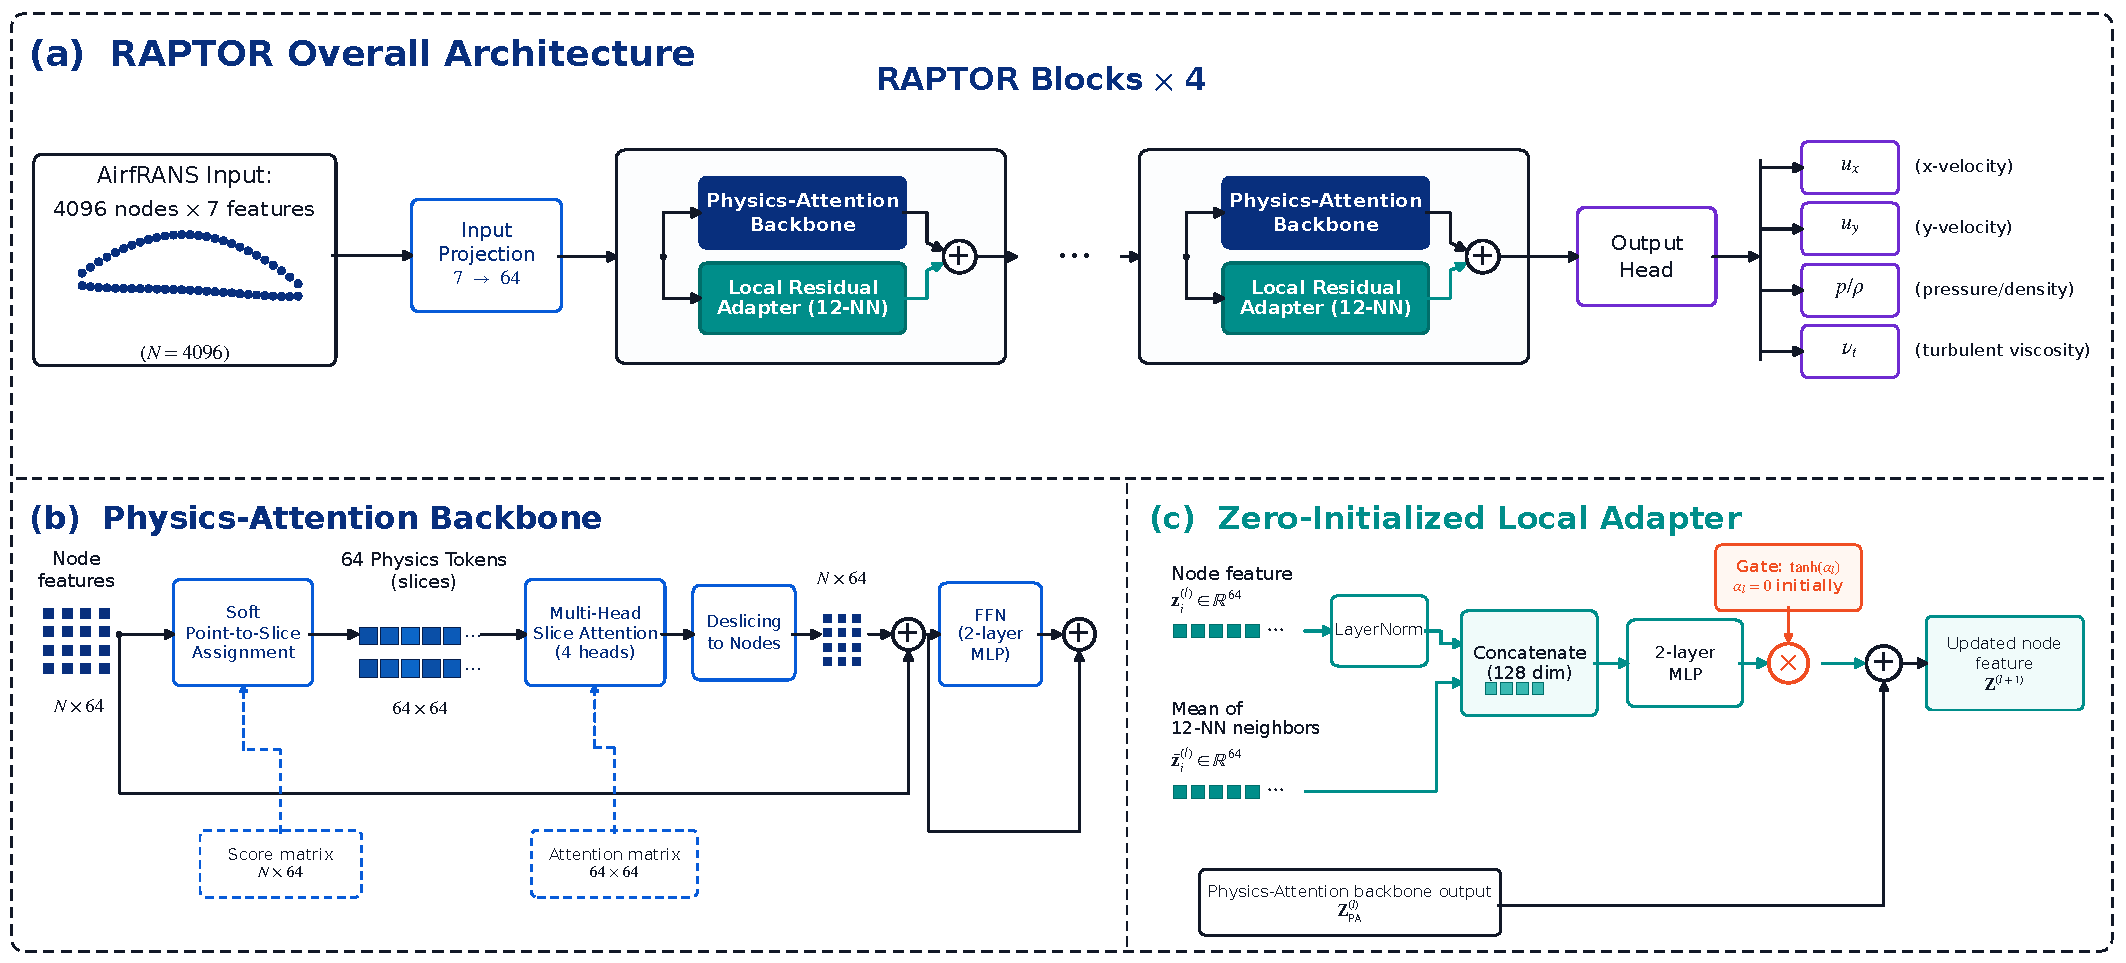
\includegraphics[
        width=\linewidth,
        keepaspectratio
	]{figs/Fig1.pdf}
    \captionof{figure}{Architecture of RAPTOR.
    (a) Overall prediction architecture illustrated using the AirfRANS configuration.  (b) Multi-head Physics-Attention backbone, which compresses node features into physics tokens, performs global token interaction, and maps the updated tokens back to the original nodes.  (c) Zero-initialized local adapter. LayerNorm is applied only to the center-node feature before it is concatenated with the unnormalized mean of its \(K\) neighbors; the resulting local message is gated and added to the Physics-Attention backbone output.}
    \label{fig1}
\end{minipage}
\end{center}
\subsection{Overall architecture}

Let an aerodynamic sample be represented by \(N\) irregularly distributed nodes with input attributes $ \mathbf{X}=[\mathbf{x}_1,\ldots,\mathbf{x}_N]^{\top}    \in\mathbb{R}^{N\times d_{\mathrm{in}}},$ where \(d_{\mathrm{in}}\) depends on the task. The raw node attributes may contain spatial coordinates, geometric descriptors, boundary information, and flow conditions. An input projection maps these heterogeneous variables into a shared \(d\)-dimensional latent space:
\begin{equation}
    \mathbf{Z}^{(0)} = \phi_{\mathrm{in}}(\mathbf{X})\in\mathbb{R}^{N\times d}.
    \label{eq:input_projection}
\end{equation}
The latent width is set to \(d=64\) in the experiments. This width provides sufficient capacity for cross-variable representation while remaining compatible with the memory constraints of the target consumer-grade GPU. The latent representation is processed by \(L\) stacked RAPTOR blocks:
\begin{equation}
    \mathbf{Z}^{(l+1)}  = \mathcal{R}^{(l)}  \left( \mathbf{Z}^{(l)},\mathcal{N}_K \right),
    \qquad l=0,\ldots,L-1,
    \label{eq:stacked_raptor}
\end{equation}
where \(\mathcal{N}_K\) denotes a fixed Euclidean \(K\)-nearest-neighbor graph constructed from the node coordinates. Self-neighbors are excluded; the queried neighborhoods are directed and are not symmetrized. The indices are precomputed once for every sampled geometry and reused throughout training and evaluation. Each block contains a Physics-Attention global backbone and a gated local residual adapter.
The final aerodynamic field is decoded as:
\begin{equation}
    \widehat{\mathbf{Y}}
    =
    \phi_{\mathrm{out}}
    \left(
        \mathbf{Z}^{(L)}
    \right)
    \in\mathbb{R}^{N\times d_{\mathrm{out}}}.
    \label{eq:output_projection}
\end{equation}

The input and output dimensions are task-dependent. For the AirfRANS experiments shown in Fig.~\ref{fig1}, \(N=4096\), \(d_{\mathrm{in}}=7\), and \(d_{\mathrm{out}}=4\). The seven inputs are the two node coordinates, two inlet-velocity components, distance to the airfoil, and two surface-normal components. The four outputs are \(u_x\), \(u_y\), pressure divided by density \(p/\rho\), and turbulent kinematic viscosity \(\nu_t\). For the three-dimensional automobile and aircraft experiments, the input is the raw three-dimensional surface coordinate and the output is the surface pressure coefficient \(C_p\). The input projection is linear. The output head applies LayerNorm, a linear layer, GELU, and a final linear layer.

\subsection{Multi-head Physics-Attention backbone}
Let \(\mathbf{Z}^{(l)}\in\mathbb{R}^{N\times d}\) denote the input to the \(l\)-th RAPTOR block. The Physics-Attention branch first applies LayerNorm and projects the normalized representation into feature and slice-assignment spaces:
\begin{equation}
    \mathbf{U}^{(l)}
    =
    \operatorname{LN}_{1}^{(l)}
    \left(
        \mathbf{Z}^{(l)}
    \right).
    \label{eq:pa_normalization}
\end{equation}

The latent dimension is divided among \(H\) attention heads, with \(d_h=d/H\). For head \(h\), the projected node and value features are:
\begin{equation}
    \mathbf{X}_{h}^{(l)}
    =
    P_{x,h}^{(l)}
    \left(
        \mathbf{U}^{(l)}
    \right),
    \qquad
    \mathbf{V}_{h}^{(l)}
    =
    P_{f,h}^{(l)}
    \left(
        \mathbf{U}^{(l)}
    \right),
    \label{eq:head_features}
\end{equation}
where
\(\mathbf{X}_{h}^{(l)},\mathbf{V}_{h}^{(l)} \in\mathbb{R}^{N\times d_h}\).

Each attention head learns its own soft point-to-slice assignment:
\begin{equation}
    \mathbf{W}_{h}^{(l)}
    =
    \operatorname{Softmax}_{S}
    \left(
        \frac{
            \mathbf{X}_{h}^{(l)}
            \mathbf{W}_{s,h}^{(l)}
        }{
            \tau_{h}^{(l)}
        }
    \right)
    \in\mathbb{R}^{N\times S},
    \label{eq:slice_assignment}
\end{equation}
where \(S\) is the number of physics slices and \(\tau_h^{(l)}\) is a learnable temperature initialized to \(0.5\) and clamped to \([0.1,5.0]\). The softmax is applied over the \(S\) slices, so that:$ w_{h,is}^{(l)}\geq 0,  \qquad \sum_{s=1}^{S}w_{h,is}^{(l)}=1.$

The mass of each physics slice is:
\begin{equation}
    d_{h,s}^{(l)}
    =
    \sum_{i=1}^{N}
    w_{h,is}^{(l)},
    \qquad
    \mathbf{D}_{h}^{(l)}
    =
    \operatorname{diag}
    \left(
        d_{h,1}^{(l)},\ldots,d_{h,S}^{(l)}
    \right).
    \label{eq:slice_mass}
\end{equation}

The node features are compressed into \(S\) physics tokens using mass-normalized aggregation:
\begin{equation}
    \mathbf{T}_{h}^{(l)}
    =
    \left(
        \mathbf{D}_{h}^{(l)}
        +\varepsilon\mathbf{I}
    \right)^{-1}
    \left(
        \mathbf{W}_{h}^{(l)}
    \right)^{\top}
    \mathbf{V}_{h}^{(l)}
    \in\mathbb{R}^{S\times d_h},
    \label{eq:token_aggregation}
\end{equation}
where \(\varepsilon>0\) prevents numerical division by zero.

Queries, keys, and values are computed in the token space:
\begin{equation}
    \mathbf{Q}_{h}^{(l)}
    =
    \mathbf{T}_{h}^{(l)}
    \mathbf{W}_{Q,h}^{(l)},
    \quad
    \mathbf{K}_{h}^{(l)}
    =
    \mathbf{T}_{h}^{(l)}
    \mathbf{W}_{K,h}^{(l)},
    \quad
    \mathbf{V}_{T,h}^{(l)}
    =
    \mathbf{T}_{h}^{(l)}
    \mathbf{W}_{V,h}^{(l)}.
    \label{eq:token_qkv}
\end{equation}

The slice-level attention matrix and updated tokens are:
\begin{equation}
    \mathbf{A}_{h}^{(l)}
    =
    \operatorname{Softmax}
    \left(
        \frac{
            \mathbf{Q}_{h}^{(l)}
            \left(
                \mathbf{K}_{h}^{(l)}
            \right)^{\top}
        }{
            \sqrt{d_h}
        }
    \right)
    \in\mathbb{R}^{S\times S},
    \label{eq:slice_attention}
\end{equation}
\begin{equation}
    \widetilde{\mathbf{T}}_{h}^{(l)}
    =
    \mathbf{A}_{h}^{(l)}
    \mathbf{V}_{T,h}^{(l)}.
    \label{eq:updated_tokens}
\end{equation}

The updated tokens are mapped back to the original nodes using the same soft assignment:
\begin{equation}
    \mathbf{G}_{h}^{(l)}
    =
    \mathbf{W}_{h}^{(l)}
    \widetilde{\mathbf{T}}_{h}^{(l)}
    \in\mathbb{R}^{N\times d_h}.
    \label{eq:deslicing}
\end{equation}
Outputs from all attention heads are concatenated and linearly projected:
\begin{equation}
    \mathbf{G}^{(l)}
    =
    P_{o}^{(l)}
    \left(
        \operatorname{Concat}
        \left[
            \mathbf{G}_{1}^{(l)},\ldots,
            \mathbf{G}_{H}^{(l)}
        \right]
    \right).
    \label{eq:multihead_output}
\end{equation}
The Physics-Attention backbone contains two residual updates. Its feed-forward network uses expansion ratio four, \(d\rightarrow4d\rightarrow d\):
\begin{equation}
    \mathbf{U}_{\mathrm{PA}}^{(l)}
    =
    \mathbf{Z}^{(l)}
    +
    \mathbf{G}^{(l)},
    \label{eq:attention_residual}
\end{equation}
\begin{equation}
    \mathbf{Z}_{\mathrm{PA}}^{(l)}
    =
    \mathbf{U}_{\mathrm{PA}}^{(l)}
    +
    \operatorname{FFN}^{(l)}
    \left(
        \operatorname{LN}_{2}^{(l)}
        \left(
            \mathbf{U}_{\mathrm{PA}}^{(l)}
        \right)
    \right).
    \label{eq:ffn_residual}
\end{equation}

Global communication is therefore performed among \(S\) physics tokens instead of directly among all \(N\) nodes. This construction avoids an explicit dense \(N\times N\) node-attention matrix while retaining a global information pathway.

\subsection{Zero-initialized local residual adapter}
Although token-mediated interaction provides an efficient global pathway, compressing \(N\) nodes into \(S\) physics tokens can weaken information associated with local surface continuity, geometric curvature, boundary layers, and sharp field variations. RAPTOR therefore introduces a sparse local adapter operating directly in the original node space. For node \(i\), let \(\mathcal{N}_K(i)\) denote the indices of its \(K\) nearest neighbors. The neighborhood feature is computed by mean aggregation:  $ \overline{\mathbf{z}}_{i}^{(l)}
    =
    \frac{1}{K}
    \sum_{j\in\mathcal{N}_K(i)}
    \mathbf{z}_{j}^{(l)}.$

Consistent with the implementation, LayerNorm is applied to the center-node feature before concatenation, while the aggregated neighborhood feature is used directly. The local message is:
\begin{equation}
    \mathbf{m}_{i}^{(l)}
    =
    \phi_{\mathrm{loc}}^{(l)}
    \left(
        \left[
            \operatorname{LN}_{\mathrm{loc}}^{(l)}
            \left(
                \mathbf{z}_{i}^{(l)}
            \right);
            \overline{\mathbf{z}}_{i}^{(l)}
        \right]
    \right),
    \label{eq:local_message}
\end{equation}
where \([\cdot\,;\cdot]\) denotes feature concatenation and \(\phi_{\mathrm{loc}}^{(l)}\) is a two-layer MLP with GELU activation and hidden width \(d\): \(2d\rightarrow d\rightarrow d\).

Collecting the node-level messages gives: $ \mathbf{M}_{\mathrm{loc}}^{(l)}  =  \left[ \mathbf{m}_{1}^{(l)},\ldots,        \mathbf{m}_{N}^{(l)}  \right]^{\top}  \in\mathbb{R}^{N\times d}.$ The local message is modulated by a learnable scalar gate: $  \gamma_l=\tanh(\alpha_l),    \qquad    -1<\gamma_l<1,$ and the output of the \(l\)-th RAPTOR block is:
\begin{equation}
    \mathbf{Z}^{(l+1)}
    =
    \mathbf{Z}_{\mathrm{PA}}^{(l)}
    +
    \tanh(\alpha_l)
    \mathbf{M}_{\mathrm{loc}}^{(l)}.
    \label{eq:raptor_block}
\end{equation}

The local adapter takes the original block input \(\mathbf{Z}^{(l)}\), whereas \(\mathbf{Z}_{\mathrm{PA}}^{(l)}\) is obtained after the Physics-Attention and feed-forward residual updates. This parallel construction preserves
the original global backbone and adds an independent local correction. Each gate is initialized as \(\alpha_l=0\). Consequently, the local branch contributes exactly zero at initialization. Its effect is activated progressively during optimization, as analyzed in Section~\ref{sec:theory}.

\subsection{Training objective and reconstruction procedure}
\label{subsec:training}
Let \(\widehat{\mathbf{Y}}^{(q)}\) and \(\mathbf{Y}^{(q)}\) denote the normalized prediction and ground-truth field of training sample \(q\). The model is trained by minimizing the node-averaged mean-squared error:
\begin{equation}
    \mathcal{L}_{\mathrm{train}}
    =
    \frac{1}{N_{\mathrm{tr}}}
    \sum_{q=1}^{N_{\mathrm{tr}}}
    \frac{1}{N_qd_{\mathrm{out}}}
    \left\|
        \widehat{\mathbf{Y}}^{(q)}
        -
        \mathbf{Y}^{(q)}
    \right\|_{F}^{2}.
    \label{eq:training_loss}
\end{equation}

Normalization statistics are computed using only the training set. For AirfRANS, all seven inputs and four outputs are standardized channel-wise. For the three-dimensional tasks, coordinates remain in their stored units and only \(C_p\) is standardized using the scalar training-set mean and standard deviation. Model selection uses validation loss with early stopping; the validation-selected checkpoint is restored for test evaluation, after which predictions are transformed back to physical units where required. Because the surrounding optimizer and early-stopping loop is standard, Algorithm~\ref{alg:raptor} separates the RAPTOR-specific setup from the repeatedly executed forward pass. \textsc{InitializeRAPTOR} is called once before optimization, \textsc{CacheKNNGraph} is called once for each sampled geometry, and \textsc{RAPTORForward} is called repeatedly during training and inference without reinitializing any parameter.

\begin{algorithm}[H]
\caption{Separated RAPTOR initialization, graph caching, and forward propagation}
\label{alg:raptor}
\footnotesize
\begin{algorithmic}[1]
\Require Sampled node features \(\mathbf X\), coordinates \(\mathbf C=\{\mathbf c_i\}_{i=1}^{N}\), fitted input preprocessor \(\mathcal P_X\), slices \(S\), neighbors \(K\), and blocks \(L\)
\Procedure{InitializeRAPTOR}{$S,L$}
    \State Initialize all non-gate trainable parameters in \(\theta\)
    \State Set \(\alpha_l\gets0\) for \(l=0,\ldots,L-1\)
    \State \Return initialized model parameters \(\theta\)
\EndProcedure
\Procedure{CacheKNNGraph}{$\mathbf C,K$}
    \ForAll{nodes \(i=1,\ldots,N\)}
        \State \(\mathcal N_K(i)\gets\operatorname{KNN}_K
        (\mathbf c_i,\{\mathbf c_j:j\ne i\})\)
    \EndFor
    \State Cache and \Return the directed, self-excluding graph \(\mathcal N_K\)
\EndProcedure
\Procedure{RAPTORForward}{$\mathbf X,\mathcal N_K;\theta$}
    \State \(\mathbf Z^{(0)}\gets\phi_{\mathrm{in}}
    \!\left(\mathcal P_X(\mathbf X)\right)\)
    \For{\(l=0,\ldots,L-1\)}
        \State \(\mathbf U_{\mathrm{PA}}^{(l)}\gets\mathbf Z^{(l)}+
        \operatorname{PhysicsAttn}^{(l)}
        \!\left(\operatorname{LN}_{1}^{(l)}(\mathbf Z^{(l)}),S\right)\)
        \State \(\mathbf Z_{\mathrm{PA}}^{(l)}\gets\mathbf U_{\mathrm{PA}}^{(l)}+
        \operatorname{FFN}^{(l)}
        \!\left(\operatorname{LN}_{2}^{(l)}(\mathbf U_{\mathrm{PA}}^{(l)})\right)\)
        \ForAll{nodes \(i=1,\ldots,N\) in parallel}
            \State \(\overline{\mathbf z}_{i}^{(l)}\gets
            K^{-1}\!\sum_{j\in\mathcal N_K(i)}\mathbf z_j^{(l)}\)
            \State \(\mathbf m_i^{(l)}\gets\phi_{\mathrm{loc}}^{(l)}
            \!\left([\operatorname{LN}_{\mathrm{loc}}^{(l)}(\mathbf z_i^{(l)});
            \overline{\mathbf z}_{i}^{(l)}]\right)\)
        \EndFor
        \State \(\mathbf M_{\mathrm{loc}}^{(l)}\gets
        [\mathbf m_1^{(l)},\ldots,\mathbf m_N^{(l)}]^{\top}\)
        \State \(\mathbf Z^{(l+1)}\gets\mathbf Z_{\mathrm{PA}}^{(l)}+
        \tanh(\alpha_l)\mathbf M_{\mathrm{loc}}^{(l)}\)
    \EndFor
    \State \(\widehat{\mathbf Y}\gets\phi_{\mathrm{out}}(\mathbf Z^{(L)})\)
    \State \Return normalized field prediction \(\widehat{\mathbf Y}\)
\EndProcedure
\end{algorithmic}
\end{algorithm}

\subsection{Connectivity and computational complexity}
\label{subsec:complexity}

Dense node-level self-attention constructs interactions between every pair of nodes. Its logical attention-score count is $|\mathcal E_{\mathrm{dense}}| = \mathcal O(HN^2),$ and principal interaction complexity is $\mathcal C_{\mathrm{dense}}
    =
    \mathcal O(N^2d),$
where \(H\) is the number of attention heads.
For RAPTOR, every attention head constructs \(NS\) point-to-slice scores and \(S^2\) slice-to-slice attention scores. The local adapter introduces \(NK\) directed neighborhood dependencies. Therefore, one RAPTOR block
has the logical interaction count $|\mathcal E_{\mathrm{RAPTOR}}| = \mathcal O \left( HNS+HS^2+NK \right).$
When \(H\) is treated as a fixed architectural constant, this reduces to $|\mathcal E_{\mathrm{RAPTOR}}|
    =
    \mathcal O
    \left(
        NS+S^2+NK
    \right).$
The interaction-related arithmetic complexity is $ \mathcal C_{\mathrm{interaction}}
    =
    \mathcal O
    \left(
        NSd+S^2d+NKd
    \right).$
Feature projections, the feed-forward network, and the two-layer local MLP additionally introduce an \(\mathcal O(Nd^2)\) term. The complete per-block complexity is therefore $\mathcal C_{\mathrm{block}}
    =
    \mathcal O
    \left(
        NSd+S^2d+NKd+Nd^2
    \right).$
For \(L\) blocks, the total complexity is $ \mathcal C_{\mathrm{RAPTOR}}
    =
    \mathcal O
    \left[
        L
        \left(
            NSd+S^2d+NKd+Nd^2
        \right)
    \right].$
When \(S\), \(K\), \(H\), \(d\), and \(L\) remain fixed, both the interaction count and arithmetic complexity grow linearly with \(N\). This statement excludes graph construction. Exact Euclidean \(K\)-NN search costs \(\mathcal{O}(N^2)\) with the pairwise implementation used for the three-dimensional caches (or approximately \(\mathcal{O}(N\log N)\) with the \(k\)-d tree used for AirfRANS), plus \(\mathcal{O}(NK)\) storage. Because graphs are precomputed, these costs are not included in the reported training time or peak allocated training memory.

Euclidean proximity is only an approximation to surface adjacency. A directed neighbor may cross a thin wing, a vehicle gap, or another nearby but geodesically distant surface. The present experiments do not prevent such connections; mesh-edge or geodesic neighborhoods are therefore an important control for future work.

\section{Theoretical Properties of RAPTOR}
\label{sec:theory}

\subsection{Conditional global mixing and sparse local support}
\label{subsec:operator_decomposition}

A RAPTOR block can be expressed as:
\begin{equation}
    \mathcal R_{\mathrm{RAPTOR}}
    \left(
        \mathbf Z,\mathcal N_K
    \right)
    =
    \mathcal P_{\mathrm{global}}(\mathbf Z)
    +
    \gamma_{\alpha}
    \mathcal A_{\mathrm{local}}
    \left(
        \mathbf Z,\mathcal N_K
    \right),
    \qquad
    \gamma_{\alpha}=\tanh(\alpha),
    \label{eq:raptor_operator_decomposition}
\end{equation}
where \(\mathcal P_{\mathrm{global}}\) is the complete Physics-Attention backbone, including its attention and feed-forward residual updates, and \(\mathcal A_{\mathrm{local}}\) is the sparse \(K\)-NN adapter.

Equation~\eqref{eq:raptor_operator_decomposition} is an architectural decomposition, not a low-rank decomposition of the complete nonlinear operator or its Jacobian. Both the point-to-slice assignment and the slice-level attention matrix depend on \(\mathbf Z\); the local branch also contains normalization, GELU, and a nonlinear MLP.

For a fixed input state, however, the node-mixing pattern of each Physics-Attention head is mediated by only \(S\) physics slices, whereas the direct dependencies of the local branch are supported on the sparse \(K\)-NN graph. RAPTOR can therefore be interpreted structurally as:
\begin{equation}
    \underbrace{
        \text{token-mediated global interaction}
    }_{\text{low-rank per attention head}}
    \quad+\quad
    \underbrace{
        \text{\(K\)-NN local correction}
    }_{\text{sparse node-level support}}.
    \label{eq:structural_interpretation}
\end{equation}

The two branches serve complementary purposes. The global branch provides communication between distant aerodynamic regions, whereas the local branch preserves neighborhood-scale geometric and physical variation.

\subsection{Conditional rank of a Physics-Attention head}
\label{subsec:rank_property}

Consider one attention head \(h\) at a fixed input state and omit the block superscript for clarity. Let $\mathbf{W}_h\in\mathbb R^{N\times S}$ denote its node-to-slice assignment and $ \mathbf{D}_h
    =
    \operatorname{diag}
    \left(
        \mathbf W_h^{\top}\mathbf 1_N
    \right)$ slice-mass matrix. Let \(\mathbf A_h\in\mathbb R^{S\times S}\) denote the corresponding slice-attention matrix. Ignoring feature projections, which act on the channel dimension rather than directly increasing the number of node-mixing modes, the effective node-space interaction of head \(h\) is:
\begin{equation}
    \mathbf K_h
    =
    \mathbf W_h
    \mathbf A_h
    \left(
        \mathbf D_h+\varepsilon\mathbf I
    \right)^{-1}
    \mathbf W_h^{\top}
    \in\mathbb R^{N\times N}.
    \label{eq:per_head_kernel}
\end{equation}

\begin{proposition}[Per-head frozen conditional rank]
\label{prop:per_head_rank}
For each Physics-Attention head \(h\), after freezing the input-dependent assignment and slice-attention matrices, the effective node-level interaction matrix in Equation~\eqref{eq:per_head_kernel} satisfies $ \operatorname{rank}(\mathbf K_h)
    \leq S.$
\end{proposition}

\begin{proof}
The matrix \(\mathbf K_h\) is a product whose node-to-slice factors have
inner dimension \(S\). Therefore,
\begin{equation}
\begin{aligned}
    \operatorname{rank}(\mathbf K_h)
    &\leq
    \operatorname{rank}(\mathbf W_h) \leq S.
\end{aligned}
\end{equation}

\end{proof}

Proposition~\ref{prop:per_head_rank} formalizes only a frozen, per-head node-mixing statement. It is not a rank bound for the complete multi-head nonlinear block or its Jacobian, because the assignments, attention matrices, concatenation, and channel-wise output projection are input dependent.

\subsection{Sparse support of the local correction}
\label{subsec:sparse_local_support}

The local adapter produces the node-level message $\mathbf m_i
    =
    \phi_{\mathrm{loc}}
    \left(
        \left[
            \operatorname{LN}(\mathbf z_i);
            \frac{1}{K}
            \sum_{j\in\mathcal N_K(i)}
            \mathbf z_j
        \right]
    \right).$
For a fixed neighborhood graph, \(\mathbf m_i\) depends directly only on the center node \(i\) and the nodes in \(\mathcal N_K(i)\). Consequently, the direct node-dependency graph contains at most \(N(K+1)\) center and
neighbor relations: $ |\mathcal E_{\mathrm{local}}|
    =
    \mathcal O(NK).$

Because \(\phi_{\mathrm{loc}}\) is nonlinear, the local adapter is not a fixed sparse linear matrix. Its sparsity refers to the support of its direct node dependencies, or equivalently to the sparsity pattern of its node-wise Jacobian for a fixed \(K\)-NN graph. This sparse support complements the token-mediated global interaction.
It introduces direct geometric communication without restoring dense node-level attention.

\subsection{Baseline recovery and progressive adapter activation}
\label{subsec:baseline_recovery}

Let
\begin{equation}
    \mathbf Z^{+}
    =
    \mathbf Z_{\mathrm{PA}}
    +
    \tanh(\alpha)\mathbf M_{\mathrm{loc}}
    \label{eq:gated_block_output}
\end{equation}

denote the output of one RAPTOR block.

\begin{proposition}[Exact backbone recovery at initialization]
\label{prop:baseline_recovery}
If the local gate is initialized as \(\alpha_0=0\), then the RAPTOR block is exactly equivalent to its Physics-Attention backbone at initialization: $ \left.
        \mathbf Z^{+}
    \right|_{\alpha=0}
    =
    \mathbf Z_{\mathrm{PA}}.$

\end{proposition}

\begin{proof}
Since \(\tanh(0)=0\), Equation~\eqref{eq:gated_block_output} gives $ \left.
        \mathbf Z^{+}
    \right|_{\alpha=0}
    =
    \mathbf Z_{\mathrm{PA}}
    +
    0\cdot\mathbf M_{\mathrm{loc}}
    =
    \mathbf Z_{\mathrm{PA}}.$
\end{proof}

The equality in Proposition~\ref{prop:baseline_recovery} is exact rather than asymptotic. If the Physics-Attention and feed-forward parameters are copied from a backbone model, RAPTOR produces identical initial outputs,
up to numerical precision. 

Although the local message does not contribute to the initial forward pass, the gate can still receive a nonzero gradient. For a scalar loss \(\mathcal L\),
\begin{equation}
    \frac{\partial\mathcal L}{\partial\alpha}
    =
    \left\langle
        \frac{\partial\mathcal L}
        {\partial\mathbf Z^{+}},
        \mathbf M_{\mathrm{loc}}
    \right\rangle_F
    \left(
        1-\tanh^2(\alpha)
    \right),
    \label{eq:gate_gradient}
\end{equation}
where \(\langle\cdot,\cdot\rangle_F\) denotes the Frobenius inner product. At initialization,
\begin{equation}
    \left.
        \frac{\partial\mathcal L}{\partial\alpha}
    \right|_{\alpha=0}
    =
    \left\langle
        \frac{\partial\mathcal L}
        {\partial\mathbf Z^{+}},
        \mathbf M_{\mathrm{loc}}
    \right\rangle_F,
    \label{eq:initial_gate_gradient}
\end{equation}
which is generally nonzero.

By contrast, if \(\vartheta_{\mathrm{loc}}\) denotes a parameter inside the local MLP, then $\left.
        \frac{\partial\mathcal L}
        {\partial\vartheta_{\mathrm{loc}}}
    \right|_{\alpha=0}
    =
    0,$
because the local message is multiplied by \(\tanh(0)=0\).

This property prevents the randomly initialized local MLP from immediately perturbing the Physics-Attention representation while still allowing the optimizer to determine whether and in which direction the local correction
should be activated.

\begin{remark}[Bounded scalar multiplier]
Because \(|\tanh(\alpha)|\leq1\),
\[
\left\|\mathbf Z^{+}-\mathbf Z_{\mathrm{PA}}\right\|_F
\leq \left\|\mathbf M_{\mathrm{loc}}\right\|_F .
\]
This direct norm inequality bounds only the scalar multiplier; it does not bound the nonlinear local message independently of the input.
\end{remark}

\begin{remark}[Conditional branch complementarity]
\label{rem:conditional_complementarity}
Suppose that an aerodynamic field contains long-range dependencies that
can be represented effectively by token-mediated global interaction and
a remaining component that is predictable from local geometric
neighborhoods. Under this condition, the Physics-Attention backbone and
the \(K\)-NN adapter provide complementary approximation mechanisms.
This interpretation explains the motivation for RAPTOR but does not
constitute a universal superiority theorem. The actual benefit of the
local branch must be established empirically through matched-baseline
comparisons and ablation experiments.
\end{remark}

\section{Experimental Setup}
\label{sec:experimental_setup}

RAPTOR is evaluated through a progression from two-dimensional airfoils
to three-dimensional automobiles and aircraft. The AirfRANS tasks assess
field reconstruction under unseen flow conditions; the automobile task
examines reconstruction on complex three-dimensional surfaces; and the aircraft task tests
applicability across distinct aerodynamic geometries. An overview of
the locally downloaded datasets is given in
Table~\ref{tab:dataset_overview}.

\subsection{Datasets}
\label{subsec:datasets}

\textbf{(1) Two-dimensional airfoils.}
The AirfRANS dataset~\citep{ref04} contains steady two-dimensional
Reynolds-averaged Navier--Stokes simulations over varying airfoil
geometries, Reynolds numbers, and angles of attack. We evaluate
Reynolds-number and angle-of-attack extrapolation using the official
task-specific partitions. For each task, 200 simulations are selected
from the official training partition with selection seed 2026 and split
into 180 training and 20 validation cases; 200 simulations are selected
from the official test partition. Each case is downsampled to
\(N=4096\) nodes using 20\% surface and 80\% volume samples. Sampling
uses deterministic split offsets 1000, 5000, and 9000 for training,
validation, and test cases, respectively. This is a custom downsampled
evaluation rather than the official full-node metric. The seven inputs
are \(x\), \(y\), the two inlet-velocity components, distance to the
airfoil, and the two normal components. Targets are \(u_x\), \(u_y\),
pressure divided by density \(p/\rho\), and turbulent kinematic
viscosity \(\nu_t\).

\textbf{(2) Three-dimensional automobiles.}
The automobile task uses the Mixed-3D benchmark~\citep{ref18,ref37}, whose
automobile geometries are derived from DrivAerNet++~\citep{ref05}. Mixed-3D
provides surface pressure coefficients \(C_p\) computed by a panel method
under the prescribed freestream \(\mathbf v_\infty=[1,0,0]\). We select
100 vehicles with seed 42, partition them into 80/10/10 training,
validation, and test objects, and sample 4096 surface nodes per object.
The model receives three-dimensional coordinates and predicts \(C_p\).

\textbf{(3) Three-dimensional aircraft.}
The aircraft task uses the OpenVSP-derived portion of Mixed-3D~\citep{ref18,ref37}
and the same panel-method \(C_p\) target. We select 25 objects from each
of the J20, P180, Boeing 737, and ERJ families with seed 42. Each family
contributes 20 training objects, while the stratified validation and test
allocations sum to 10 objects each. Every surface is sampled to 4096 nodes.
The complete automobile and aircraft object identifiers are supplied in
the accompanying split-manifest files.

% Preamble: \usepackage{booktabs,hyperref}

\begin{table}[t]
	\centering
	\caption{Locally downloaded aerodynamic datasets.
		Sizes are uncompressed and reported in decimal GB.}
	\label{tab:dataset_overview}
	\small
	\renewcommand{\arraystretch}{1.15}
	\setlength{\tabcolsep}{5pt}
	\begin{tabular}{@{}lrlrl@{}}
		\toprule
		Dataset & Samples & Task or geometry family & Size (GB) & Source \\
		\midrule
		AirfRANS
		& 1,000
		& Reynolds and AoA extrapolation
		& 15.03
		& \href{https://github.com/Extrality/AirfRANS}{AirfRANS} \\
		
		Cars
		& 5,428
		& Estateback, Fastback, Notchback
		& 4.81
		& \shortstack[l]{
			\href{https://github.com/PKU-CMEGroup/NeuralOperator}{Mixed-3D}; automobiles derived\\
			from \href{https://dataverse.harvard.edu/dataverse/DrivAerNet}{DrivAerNet++}
		} \\
		
		Aircraft
		& 6,766
		& J20, P180, Boeing 737, ERJ
		& 6.13
		& \href{https://github.com/PKU-CMEGroup/NeuralOperator}{Mixed-3D benchmark} \\
		\bottomrule
	\end{tabular}
\end{table}



\subsection{Comparison baselines}
\label{subsec:baselines}

The AirfRANS comparison includes an independent-node MLP; PointNet, GraphSAGE,
and Graph U-Net geometric baselines~\citep{ref11,ref12,ref13}; a controlled
Sparse Token implementation inspired by SEA~\citep{ref36}; and four compact
operator baselines. All ``Tiny'' operators use the common width, depth, and
latent-state budget in Table~\ref{tab:training_protocol}. Transolver-Tiny
implements Physics-Attention and is RAPTOR's direct no-adapter backbone
baseline~\citep{ref20}. Transolver++-Tiny retains point-dependent temperature
and slice reparameterization~\citep{ref21}; LinearNO-Tiny uses asymmetric
linear attention~\citep{ref22}; and MoNo-Tiny retains hierarchical latent
modes with balanced assignment~\citep{ref23}. These are resource-matched
implementations rather than the full-scale configurations of the original
studies.

The automobile experiment uses PointNet and Transolver-Tiny as primary
baselines. The aircraft evaluation compares RAPTOR with Transolver-Tiny under the same
stratified split. Because both models are retrained and all four families
occur in training and test sets, this experiment assesses applicability
across aircraft geometries rather than transfer learning or unseen-family
extrapolation.

\subsection{Unified experimental protocol}
\label{subsec:protocol}

All formal training and evaluation runs are conducted on a Windows-based laptop equipped with an Intel Core Ultra 9 185H CPU, 32~GB of system memory (31.5~GB usable), and a single NVIDIA GeForce RTX 4050 Laptop GPU with 6141~MiB of device memory. The recorded NVIDIA driver version is 596.58. The software environment uses Python 3.12.13, PyTorch 2.5.1, CUDA 12.1, NumPy 2.3.1, and SciPy 1.16.0.
The unified hyperparameter configuration is summarized in Table~\ref{tab:training_protocol}.

CUDA automatic mixed precision is enabled for the AirfRANS and
three-dimensional runs. The mixed-feature scatter in MoNo-Tiny and the
eidetic slicing operation in Transolver++-Tiny are explicitly evaluated
in FP32 because their corresponding kernels were not autocast safe.
All formal experiments use training seed 42. The two three-dimensional
split manifests record every object identifier and the sampling seed.

\paragraph{Node-scaling profiling protocol.}
Computational scaling is evaluated without retraining by applying the actual
Transolver-Tiny and RAPTOR implementations to deterministic synthetic tensors
with three input channels and one output channel. An explicit dense
node-attention baseline materializes the per-head \(N\times N\) attention
matrix. The node count is varied over
\(N\in\{1024,2048,4096,8192,16384\}\), while the number of physics slices
\(S=64\), neighborhood size \(K=12\), hidden width \(d=64\), number of
blocks \(L=4\), number of heads \(H=4\), and batch size one remain fixed.
All model measurements use CUDA AMP, 10 warm-up iterations, and 30 measured
iterations with CUDA-event timing. Each model, node count, and execution
phase is evaluated in an isolated process.

RAPTOR receives precomputed deterministic neighbor indices during the
forward and training-step measurements, so graph construction is excluded
from model latency and GPU-memory statistics. To expose that omitted cost,
the exact three-dimensional graph builder based on CPU
\texttt{torch.cdist} followed by \texttt{topk} is profiled separately using
one warm-up run, ten measured runs at each node count, and eight CPU
threads. Model-latency statistics are computed from 30 timed iterations,
whereas the \(K\)-NN statistics are computed from 10 timed runs.
\mbox{Reported error bars represent one sample standard deviation.} Peak memory denotes
the maximum CUDA allocation observed during the measured phase. 

\begin{center}
    \begin{minipage}{0.88\linewidth}
        \centering
        \captionof{table}{Common training configuration for the formal experiments.}
    \label{tab:training_protocol}
    \renewcommand{\arraystretch}{1.12}
    \setlength{\tabcolsep}{5pt}
    \begin{tabular}{lc}
        \toprule
        Setting & Value \\
        \midrule
        Training seed & 42 \\
        AirfRANS data-selection seed & 2026 \\
        Nodes per sample & 4096 \\
        Hidden dimension & 64 \\
        Number of operator blocks & 4 \\
        Number of attention heads & 4 \\
        Physics slices or latent states & 64 \\
        FFN expansion ratio & 4 \\
        Local MLP hidden width & 64 \\
        Slice-temperature initialization & 0.5 \\
        Slice-temperature bounds & \([0.1,5.0]\) \\
        RAPTOR neighborhood size \(K\) & 12 \\
        RAPTOR gate initialization & \(\alpha_l=0\) \\
        Optimizer & AdamW \\
        Initial learning rate & \(1\times10^{-3}\) \\
        Weight decay & \(1\times10^{-6}\) \\
        Maximum epochs & 100 \\
        Early-stopping patience & 15 epochs \\
        Gradient clipping & 1.0 \\
        Effective batch size & 1 sample \\
        Mixed precision & CUDA AMP; unsafe baseline kernels forced to FP32 \\
        \bottomrule
    \end{tabular}
    \end{minipage}
\end{center}

\subsection{Evaluation metrics}
\label{subsec:evaluation_metrics}

For AirfRANS, prediction accuracy is measured using one dataset-level relative
\(L_2\) error for each physical variable. For channel \(c\), predictions and
targets are concatenated over the \(M\) test cases (each containing \(N\)
sampled nodes), giving

\begin{equation}
    \varepsilon_c
    =
    \frac{
        \sqrt{\displaystyle\sum_{m=1}^{M}
        \left\|\widehat{\mathbf Y}^{(m)}_c-\mathbf Y^{(m)}_c\right\|_2^2}
    }{
        \sqrt{\displaystyle\sum_{m=1}^{M}
        \left\|\mathbf Y^{(m)}_c\right\|_2^2}+10^{-12}
    },
    \qquad
    c\in\{u_x,u_y,p/\rho,\nu_t\}.
    \label{eq:relative_l2_metric}
\end{equation}

The four-variable macro error is defined as

\begin{equation}
    \varepsilon_{\mathrm{macro}}
    =
    \frac{1}{4}
    \left(
        \varepsilon_{u_x}
        +
        \varepsilon_{u_y}
        +
        \varepsilon_{p/\rho}
        +
        \varepsilon_{\nu_t}
    \right).
    \label{eq:macro_error}
\end{equation}

For the representative \(p/\rho\) visualizations, the sample-level pressure
error of model \(a\) on test case \(q\) is
\begin{equation}
    e_{q,p}^{(a)}=
    \frac{\left\|\widehat{\mathbf Y}_{q,p}^{(a)}-\mathbf Y_{q,p}\right\|_2}
    {\left\|\mathbf Y_{q,p}\right\|_2+10^{-12}}.
    \label{eq:sample_pressure_error}
\end{equation}
Let \(R\) denote RAPTOR and \(b\) the other model displayed in the same
row. The test-set and sample-level paired pressure improvements, and the
representative-case rule, are
\begin{equation}
    \Delta_p^{\mathrm{test}}=1-\frac{\varepsilon_p^{(R)}}{\varepsilon_p^{(b)}},
    \qquad
    \Delta_{q,p}=1-\frac{e_{q,p}^{(R)}}{e_{q,p}^{(b)}},
    \qquad
    q^*=\operatorname*{arg\,min}_{q}
    \left|\Delta_{q,p}-\Delta_p^{\mathrm{test}}\right|.
    \label{eq:pressure_case_selection}
\end{equation}
Both \(e_{q,p}^{(a)}\) and \(\varepsilon_p^{(a)}\) use all 4096 sampled
nodes. The percentile-based normalization in the absolute-error maps is used
only for visualization and does not enter the selection rule. Reported
implementation measurements
comprise trainable parameters, elapsed training time, and peak allocated GPU
memory. End-to-end inference latency was not retained consistently for the
accuracy experiments and is therefore not compared across trained runs.
The separate node-scaling experiment instead reports isolated forward-pass
and complete AdamW training-step latency, excluding data loading,
post-processing, and \(K\)-NN graph construction.

For the automobile and aircraft experiments, the principal metric is ordinary
MSE after standardizing \(C_p\) with the training-set mean and standard
deviation. To distinguish it from the conventional ratio
\(\mathrm{MSE}/\|Y\|_2^2\), we call it standardized-space MSE (sMSE):

\begin{equation}
    \mathrm{sMSE}
    =
    \frac{1}{|\mathcal D_{\mathrm{te}}|}
    \sum_{m\in\mathcal D_{\mathrm{te}}}
    \frac{1}{N}
    \left\|
        \widehat{\mathbf Y}^{(m)}_{\mathrm{norm}}
        -
        \mathbf Y^{(m)}_{\mathrm{norm}}
    \right\|_F^2 .
    \label{eq:surface_standardized_mse}
\end{equation}

The best validation sMSE, training time, peak allocated GPU memory, and
parameter count are recorded together with the test result. Per-object
errors are additionally calculated to determine whether the overall
improvement is consistently distributed across geometries rather than being
dominated by a small number of test samples.

\section{Experimental Results and Analysis}
\label{sec:results}

This section evaluates RAPTOR from five complementary perspectives:
two-dimensional aerodynamic extrapolation, the contribution of the local
adapter and its initialization, three-dimensional automobile \(C_p\)
reconstruction, evaluation on aircraft geometries, and empirical node
scaling. Owing to the computational cost of the complete experimental suite,
all formal models are trained with one fixed seed (42). The complete code, configurations, split manifests, checkpoints, per-sample predictions, and evaluation scripts are available through the GitHub repository listed on the title page.

\subsection{AirfRANS extrapolation results}
\label{subsec:airfrans_results}

\subsubsection{Overall comparison}

Tables~\ref{tab:reynolds_results} and~\ref{tab:aoa_results} report the
relative \(L_2\) errors on the Reynolds-number and angle-of-attack
extrapolation tasks, respectively. The macro error is the unweighted mean
of the errors for \(u_x\), \(u_y\), \(p/\rho\), and \(\nu_t\).



On Reynolds-number extrapolation, RAPTOR has the lowest macro relative
\(L_2\) error (0.2219), improving on the nearest baseline, Transolver-Tiny
(0.2280), by 2.68\%. It is best for \(u_x\) and \(\nu_t\), whereas
Transolver-Tiny and MoNo-Tiny lead for \(u_y\) and \(p/\rho\), respectively.
The macro advantage therefore reflects balanced errors rather than dominance
on every output.

\begin{center}
    \begin{minipage}{1.00\linewidth}
        \centering
        \captionof{table}{Relative \(L_2\) errors on the AirfRANS Reynolds-number
    extrapolation task with seed 42. The upper and middle groups contain
    conventional and modern baselines, respectively. The last column
    reports the relative macro-error reduction achieved by RAPTOR over
    each baseline. The best and second-best results are shown in bold
    and underlined, respectively. Displayed errors are rounded to four
    decimals; percentages are computed from unrounded values.}
    \label{tab:reynolds_results}
    
    \renewcommand{\arraystretch}{1.12}
    \setlength{\tabcolsep}{4.5pt}
    \small
    
    \begin{tabular}{@{}lccccc@{\hspace{8pt}}c@{}}
        \toprule
        Method
        & \(u_x\)
        & \(u_y\)
        & \(p/\rho\)
        & \(\nu_t\)
        & Macro
        & \shortstack{Relative\\improvement} \\
        \midrule
        
%        \multicolumn{7}{l}{\textit{Conventional baselines}}\\[-2pt]
        
        MLP
        & 0.2713
        & 0.3892
        & 0.5578
        & 0.5127
        & 0.4327
        & 48.72\% \\
        
        GraphSAGE
        & 0.2319
        & 0.4269
        & 0.5654
        & 0.5185
        & 0.4357
        & 49.07\% \\
        
        PointNet
        & 0.2050
        & 0.2877
        & 0.2338
        & 0.3173
        & 0.2610
        & 14.98\% \\
        
        Graph U-Net
        & 0.2255
        & 0.2784
        & 0.3022
        & 0.4797
        & 0.3214
        & 30.96\% \\
        
        \midrule
%        \multicolumn{7}{l}{\textit{Modern baselines}}\\[-2pt]
        
        Sparse Token
        & 0.2412
        & 0.3309
        & 0.4034
        & 0.5043
        & 0.3699
        & 40.01\% \\
        
        Transolver-Tiny
        & \underline{0.1516}
        & \textbf{0.2233}
        & 0.2366
        & \underline{0.3003}
        & \underline{0.2280}
        & 2.68\% \\
        
        Transolver++-Tiny
        & 0.1684
        & 0.2373
        & 0.3434
        & 0.3517
        & 0.2752
        & 19.37\% \\
        
        MoNo-Tiny
        & 0.2825
        & 0.5035
        & \textbf{0.2150}
        & 0.3612
        & 0.3406
        & 34.85\% \\
        
        LinearNO-Tiny
        & 0.1565
        & \underline{0.2249}
        & 0.2360
        & 0.5360
        & 0.2884
        & 23.06\% \\
        
        \midrule
        
        \textbf{RAPTOR (ours)}
        & \textbf{0.1395}
        & 0.2292
        & \underline{0.2251}
        & \textbf{0.2939}
        & \textbf{0.2219}
        & -- \\
        
        \bottomrule
    \end{tabular}
    
    \vspace{2pt}
    \begin{minipage}{0.98\linewidth}
        \footnotesize
        \textit{Note:} Relative improvement is computed as
        \(\left(E_{\mathrm{baseline}}-E_{\mathrm{RAPTOR}}\right)/
        E_{\mathrm{baseline}}\times100\%\), where \(E\) denotes the
        macro relative \(L_2\) error. 
    \end{minipage}
    \end{minipage}
\end{center}



On AoA extrapolation, RAPTOR again obtains the lowest macro
error, 0.2969. It improves upon Transolver-Tiny by 5.37\%, showing that the
local adapter helps the Physics-Attention backbone accommodate changes in
the stagnation region, \(p/\rho\) distribution, and wake direction induced by
unseen angles of attack.

However, the advantage over LinearNO-Tiny is only 0.37\%. The two methods
should therefore be regarded as closely matched under this single-seed
protocol. LinearNO-Tiny obtains the lowest \(u_x\) error, whereas RAPTOR
performs best for \(u_y\). PointNet remains strongest for \(p/\rho\) and
turbulent viscosity. RAPTOR achieves the lowest macro error because it
avoids a large error in any one variable, rather than because it is uniformly
best on all four channels.

Across both tasks, the mean of the two macro errors is 0.2594 for RAPTOR,
compared with 0.2709 for Transolver-Tiny, 0.2932 for LinearNO-Tiny, and
0.2968 for PointNet. Under this fixed protocol, token-mediated interaction
and node-level adaptation yield the lowest two-task mean. The small AoA
margin and the use of one training seed preclude a claim of statistically
established superiority.

\begin{center}
    \begin{minipage}{1.00\linewidth}
        \centering
        \captionof{table}{Relative \(L_2\) errors on the AirfRANS angle-of-attack (AoA)
    extrapolation task with seed 42. Displayed errors are rounded to four
    decimals; percentages are computed from unrounded values.}
    \label{tab:aoa_results}
    
    \renewcommand{\arraystretch}{1.12}
    \setlength{\tabcolsep}{4.5pt}
    \small
    
    \begin{tabular}{@{}lccccc@{\hspace{8pt}}c@{}}
        \toprule
        Method
        & \(u_x\)
        & \(u_y\)
        & \(p/\rho\)
        & \(\nu_t\)
        & Macro
        & \shortstack{Relative\\improvement} \\
        \midrule
        
%        \multicolumn{7}{l}{\textit{Conventional baselines}}\\[-2pt]
        
        MLP
        & 0.3183
        & 0.4498
        & 0.6697
        & 0.5652
        & 0.5008
        & 40.71\% \\
        
        GraphSAGE
        & 0.2365
        & 0.4086
        & 0.5534
        & 0.5420
        & 0.4351
        & 31.76\% \\
        
        PointNet
        & 0.2433
        & 0.3254
        & \textbf{0.3257}
        & \textbf{0.4357}
        & 0.3326
        & 10.71\% \\
        
        Graph U-Net
        & 0.2224
        & 0.3105
        & 0.4030
        & 0.5209
        & 0.3642
        & 18.47\% \\
        
        \midrule
%        \multicolumn{7}{l}{\textit{Modern baselines}}\\[-2pt]
        
        Sparse Token 
        & 0.2993
        & 0.3267
        & 0.4576
        & 0.5982
        & 0.4204
        & 29.37\% \\
        
        Transolver-Tiny 
        & 0.1698
        & 0.2446
        & 0.3731
        & \underline{0.4676}
        & 0.3138
        & 5.37\% \\
        
        Transolver++-Tiny
        & 0.2317
        & 0.3340
        & 0.4456
        & 0.5049
        & 0.3790
        & 21.66\% \\
        
        MoNo-Tiny
        & 0.3286
        & 0.5273
        & 0.3542
        & 0.6127
        & 0.4557
        & 34.84\% \\
        
        LinearNO-Tiny
        & \textbf{0.1416}
        & \underline{0.2272}
        & 0.3512
        & 0.4720
        & \underline{0.2980}
        & 0.37\% \\
        
        \midrule
        
        \textbf{RAPTOR (ours)}
        & \underline{0.1510}
        & \textbf{0.2189}
        & \underline{0.3350}
        & 0.4828
        & \textbf{0.2969}
        & -- \\
        \bottomrule
    \end{tabular}
       \end{minipage}
\end{center}

\subsubsection{Contribution of the local adapter and gate initialization}
\label{subsec:ablation_results}

To separate the effects of local correction and gate initialization, the
complete RAPTOR model is compared with two variants: RAPTOR without the
local adapter and RAPTOR with the adapter gate initialized to
\(\alpha_l=0.1\). The complete model uses the proposed zero initialization
\(\alpha_l=0\), as reported in Table~\ref{tab:airfrans_ablation}.

\begin{center}
    \begin{minipage}{0.76\linewidth}
        \centering
        \captionof{table}{Core ablation results on AirfRANS. Values are four-variable
		macro relative $L_2$ errors. Percentages reported in the text are
		computed from unrounded values. The no-adapter entries correspond to
		the Transolver-Tiny backbone reported in Tables~3 and~4.}
	\label{tab:airfrans_ablation}
	\begin{tabular}{lcc}
		\toprule
		Variant & Reynolds & AoA \\
		\midrule
		Without local adapter
		& 0.2280
		& 0.31377 \\
		Nonzero initialization, $\alpha_l=0.1$
		& 0.24556
		& 0.32218 \\
		RAPTOR, $\alpha_l=0$
		& \textbf{0.22192}
		& \textbf{0.29692} \\
		\bottomrule
	\end{tabular}
    \end{minipage}
\end{center}


On the Reynolds-number task, RAPTOR improves by 9.63\% relative to the
nonzero-initialization variant. For Reynolds-number extrapolation, the Transolver-Tiny result reported in Table~\ref{tab:reynolds_results} (0.2280) is included as an independently trained no-adapter backbone reference, rather than as a seed-matched paired ablation. By contrast, the AoA no-adapter result is obtained from the matched ablation run. On the AoA task, RAPTOR improves by 5.37\% relative to the matched
no-adapter backbone and by 7.84\% relative to nonzero initialization. The
table reports macro errors only; variable-wise ablation percentages are not
claimed because matched per-variable results are not included.

The comparison between zero and nonzero initialization supports the
baseline-preserving role of the proposed gate. Starting from
\(\tanh(\alpha_l)=0\) allows the model to begin from the unperturbed
Physics-Attention function and to activate local corrections only when they
are supported by the optimization signal. Initializing the adapter with a
nonzero contribution degrades both extrapolation tasks. This result is
consistent with the intended optimization mechanism, although it does not
by itself constitute a general convergence guarantee.

For Reynolds extrapolation, the four learned values of
\(\tanh(\alpha_l)\) are approximately \(-0.308\), \(-0.168\), \(0.141\),
and \(0.255\). Their signs alone cannot be interpreted as reinforcement or
suppression because \(\gamma_l\mathbf M_l\) has a sign--scale
non-identifiability: the local MLP can reverse or rescale its output. A more
meaningful diagnostic is
\(\|\gamma_l\mathbf M_l\|_F/\|\mathbf Z_{\mathrm{PA}}^{(l)}\|_F\), which
should be logged in future multi-seed runs.


Figure~\ref{fig2} compares the \(p/\rho\) ground truth
and the normalized absolute \(p/\rho\) errors of the two best-performing
models on the AirfRANS extrapolation tasks. The upper and lower rows
correspond to Reynolds-number and angle-of-attack extrapolation,
respectively. The displayed models are ranked by four-variable macro relative
\(L_2\) error; the rank-2 comparators are Transolver-Tiny for Reynolds-number
extrapolation and LinearNO-Tiny for angle-of-attack extrapolation. Following
Eq.~\eqref{eq:pressure_case_selection}, test indices 165 and 142 are selected
because their paired \(p/\rho\) improvements are closest to the corresponding
pooled test-set pressure improvements. The target/selected improvements are
\(4.84\%/4.97\%\) for Reynolds-number extrapolation and
\(4.63\%/4.17\%\) for angle-of-attack extrapolation. Thus, the selection and
panel annotations use the same pressure relative \(L_2\) metric and the same
4096-node scope.
\begin{center}
	\begin{minipage}{0.94\linewidth}
		\centering
		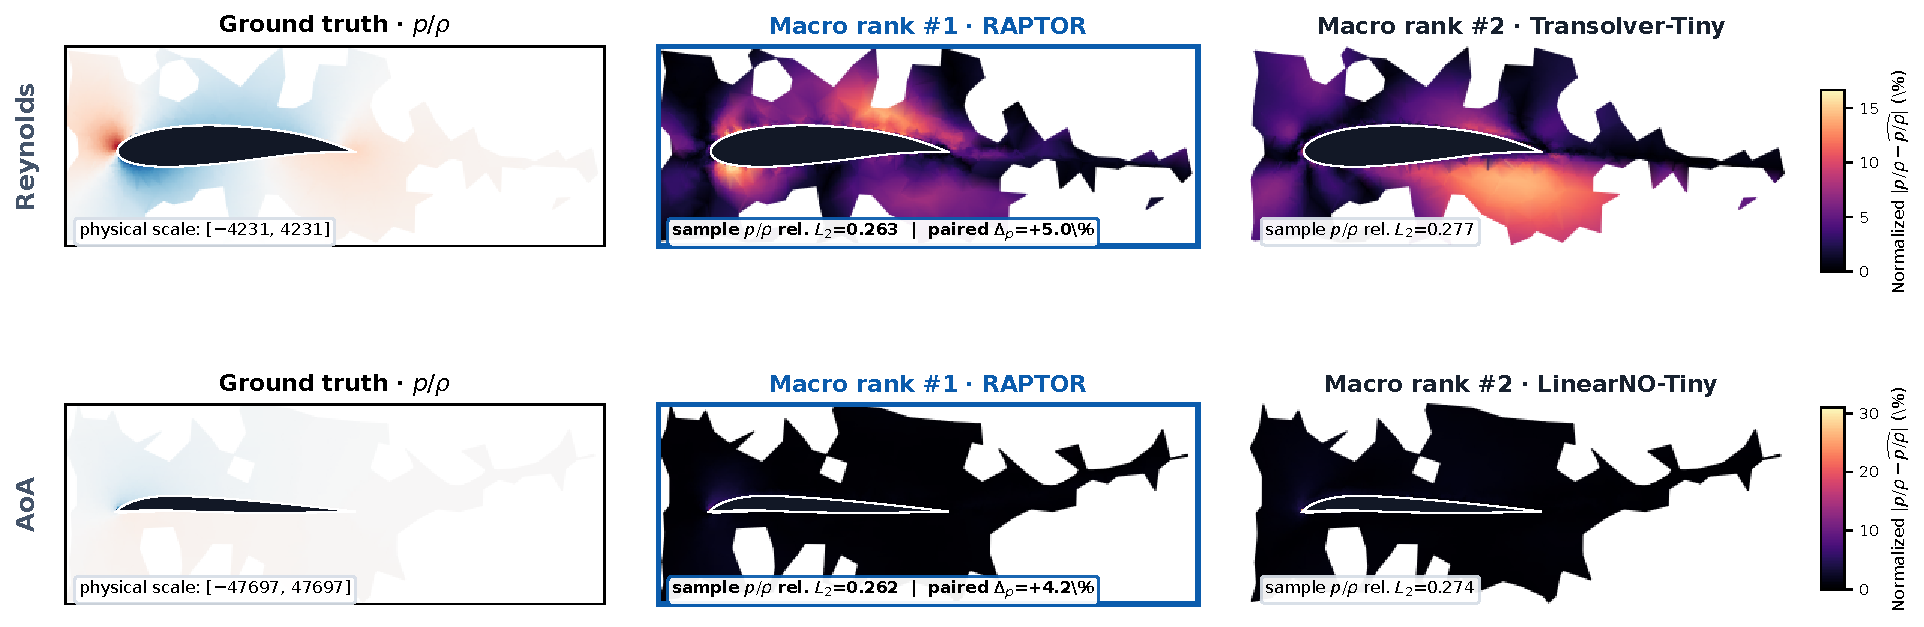
\includegraphics[
		width=\linewidth,
		keepaspectratio
		]{figs/Fig2.pdf}
		\captionof{figure}{Ground truth and normalized absolute-error maps for
			\(p/\rho\) on AirfRANS with seed 42. The Reynolds-number and AoA rows
			show test indices 165 and 142, respectively. Each case minimizes the
			difference between its sample-level paired pressure improvement and the
			corresponding pooled test-set pressure improvement, as defined in
			Eq.~\eqref{eq:pressure_case_selection}. Relative \(L_2\) errors use all
			4096 nodes; percentile normalization is applied only to the displayed
			absolute-error colors.}
		\label{fig2}
	\end{minipage}
\end{center}
\subsubsection{Representative \(p/\rho\)-error maps}
For Reynolds-number extrapolation, RAPTOR achieves a macro error of 0.222,
compared with 0.228 for Transolver-Tiny. On the displayed sample, its \(p/\rho\)
relative $L_2$ error decreases from 0.277 to 0.263, corresponding to a
$4.97\%$ improvement. This closely tracks the pooled test-set pressure
improvement of $4.84\%$ and avoids selecting an unusually favorable case.
The error maps show that the remaining deviations are concentrated near the
airfoil surface and in the downstream wake.

For angle-of-attack extrapolation, RAPTOR and LinearNO-Tiny obtain macro
errors of 0.297 and 0.298, respectively. Their overall results are therefore
close. On the representative sample, RAPTOR reduces the \(p/\rho\) relative
$L_2$ error from 0.274 to 0.262, a $4.17\%$ improvement compared with the
pooled test-set pressure improvement of $4.63\%$. The error maps indicate
that the residual differences are most visible around the leading-edge
region, the near-surface flow, and the wake.

\subsection{Three-dimensional automobile \(C_p\) reconstruction}
\label{subsec:automobile_results}

Table~\ref{tab:automobile_results} presents the results for the 100-vehicle
experiment. Transolver-Tiny is the matched no-adapter baseline.

\begin{table}[!htbp]
    \centering
    \caption{Results for the 100-vehicle surface-pressure-coefficient
    reconstruction experiment.}
    \label{tab:automobile_results}
    \renewcommand{\arraystretch}{1.10}
    \setlength{\tabcolsep}{4pt}
    \begin{tabular}{lrrrr}
        \toprule
        Model
        & Test sMSE
        & Parameters
        & Peak memory
        & Training time \\
        &
        &
        & (MiB)
        & (s) \\
        \midrule
        PointNet
        & 0.486309 & 21,057  & 23.95  & 2937.5 \\
        Transolver-Tiny
        & 0.145534 & 195,345 & 103.76 & 2428.9 \\
        RAPTOR
        & \textbf{0.135684} & 245,525 & 117.77 & 3317.2 \\
        \bottomrule
    \end{tabular}
\end{table}

RAPTOR reduces the overall test sMSE from 0.145534 for
Transolver-Tiny to 0.135684, an aggregate relative reduction of 6.77\%.
Compared with PointNet, the reduction is 72.10\%. These results suggest that
global token interaction is important for the three-dimensional
variable-geometry problem and that local adaptation provides a further improvement
over the global backbone.

The per-object comparison shows that RAPTOR
outperforms Transolver-Tiny on seven of the ten test vehicles. The mean
paired improvement is 6.16\%, the median paired improvement is 4.81\%, and
the bootstrap 95\% confidence interval is \([0.61,12.43]\%\). The positive
interval describes resampling variation among these ten fixed test objects
only; it does not include training-seed uncertainty and should not be read
as a population-level significance claim.

\begin{center}
	\begin{minipage}{0.94\linewidth}
		\centering
		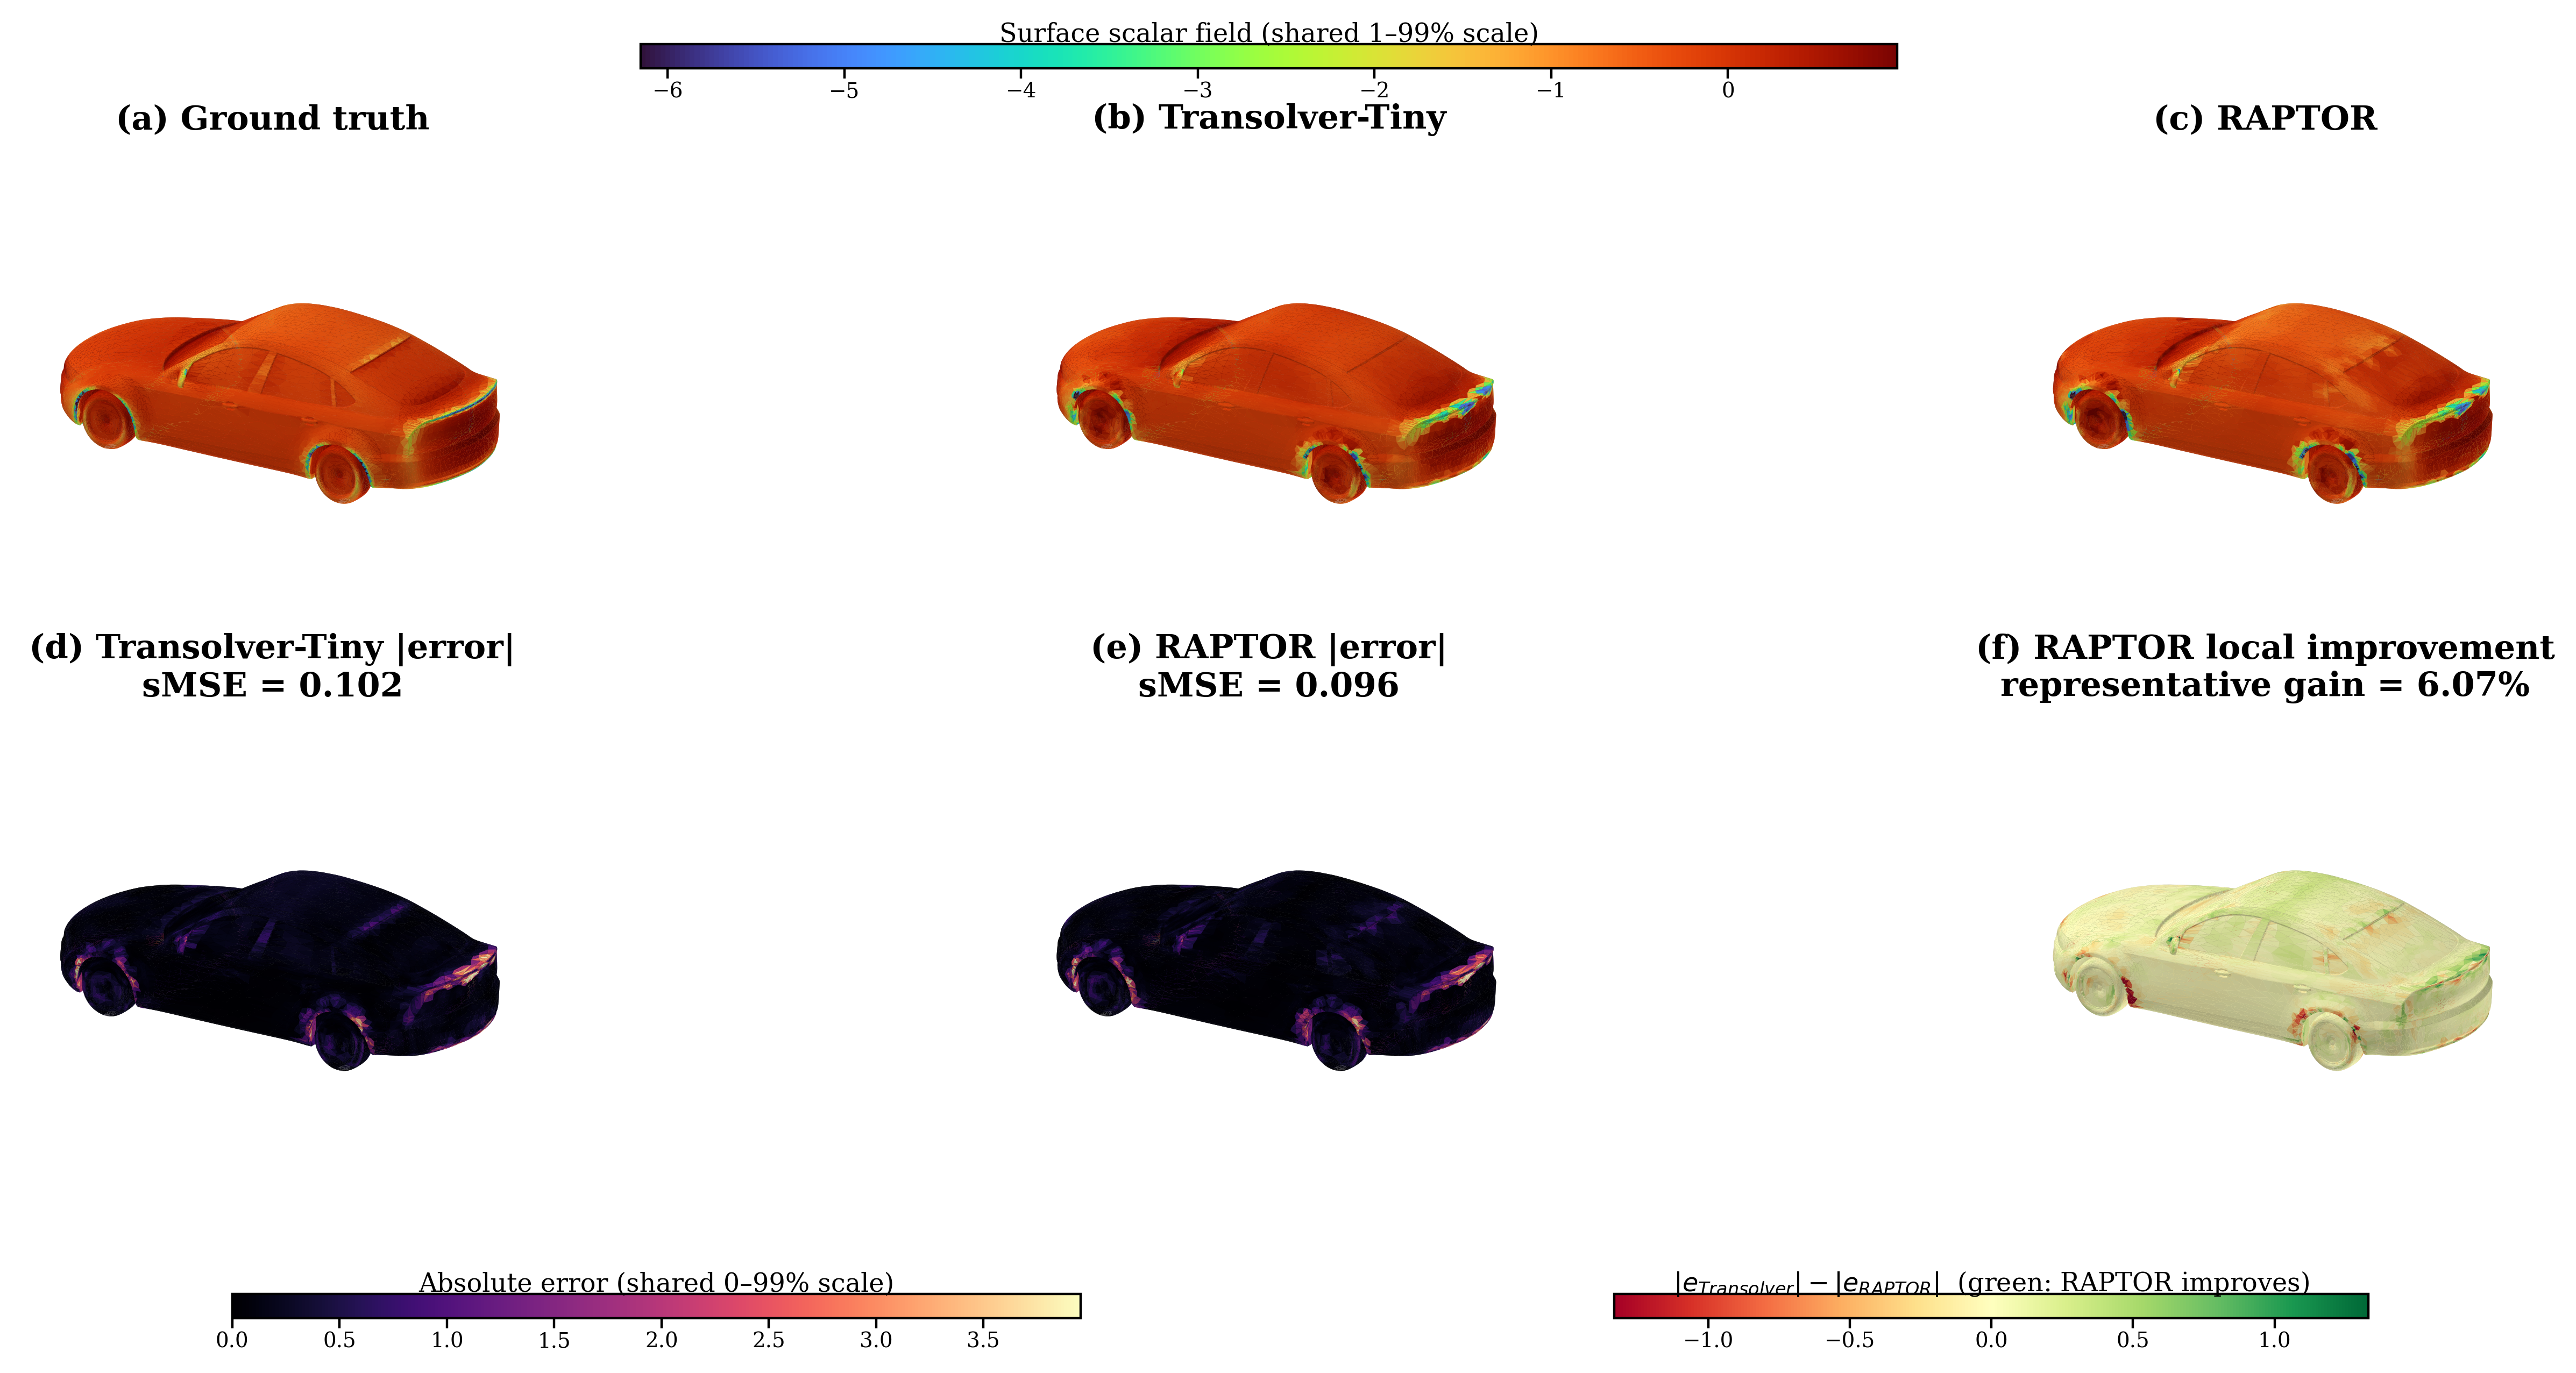
\includegraphics[
		width=\linewidth,
		keepaspectratio
		]{figs/Fig3.png}
		\captionof{figure}{Automotive \(C_p\) reconstruction and spatial error reduction
				of RAPTOR relative to Transolver-Tiny.}
		\label{fig3}
	\end{minipage}
\end{center}

Figure~\ref{fig3} compares the full-mesh
\(C_p\) reconstruction and spatial error distributions of
Transolver-Tiny and RAPTOR on a representative test vehicle. The sample
is selected according to the median vehicle-level improvement of RAPTOR,
rather than the maximum-gain case. The ground truth and two predictions
in Figs.~\ref{fig3}(a)--(c) share the same
1--99\% field scale. Both models recover the dominant \(C_p\)
distribution, while RAPTOR more closely reproduces the localized
variations around the wheels, lower body, and rear geometric edges.

Figures~\ref{fig3}(d) and
\ref{fig3}(e) show the absolute errors of
Transolver-Tiny and RAPTOR under a shared error scale. Their sMSEs are
0.10201 and 0.09582, respectively, corresponding to a 6.07\%
reduction for RAPTOR. The improvement map in
Fig.~\ref{fig3}(f) is defined as $\Delta e(\mathbf{x})
=
\left|y(\mathbf{x})-\widehat{y}_{\mathrm{Transolver}}(\mathbf{x})\right|
-
\left|y(\mathbf{x})-\widehat{y}_{\mathrm{RAPTOR}}(\mathbf{x})\right|.$

Positive green regions indicate lower errors for RAPTOR, whereas negative
red regions indicate local degradation. The distributed green regions
suggest that the improvement is associated with neighborhood-scale
corrections over several parts of the vehicle surface, particularly near
geometric edges and wheel-related structures. Small red regions also show
that the local adapter does not improve every surface location.

For visualization, predictions at the original 4,096 sampled nodes are
mapped to the full triangular mesh by nearest-neighbor interpolation.
All reported sMSE values are computed on the original sampled nodes and
are therefore unaffected by this visualization-only interpolation.



To determine where the adapter is beneficial, each vehicle is partitioned
using its own coordinate percentiles. Front and rear contain nodes below the
20th and above the 80th percentile of \(x\), respectively. Within the middle
60\%, roof contains nodes at or above the 70th percentile of \(z\),
lower/wheel-zone contains nodes at or below the 25th percentile, and side is
the remainder. A regional sMSE is first averaged over nodes within each
vehicle; Figure~\ref{fig4} reports the unweighted mean of the ten vehicle-level
regional errors.


\begin{center}
	\begin{minipage}{0.94\linewidth}
		\centering
		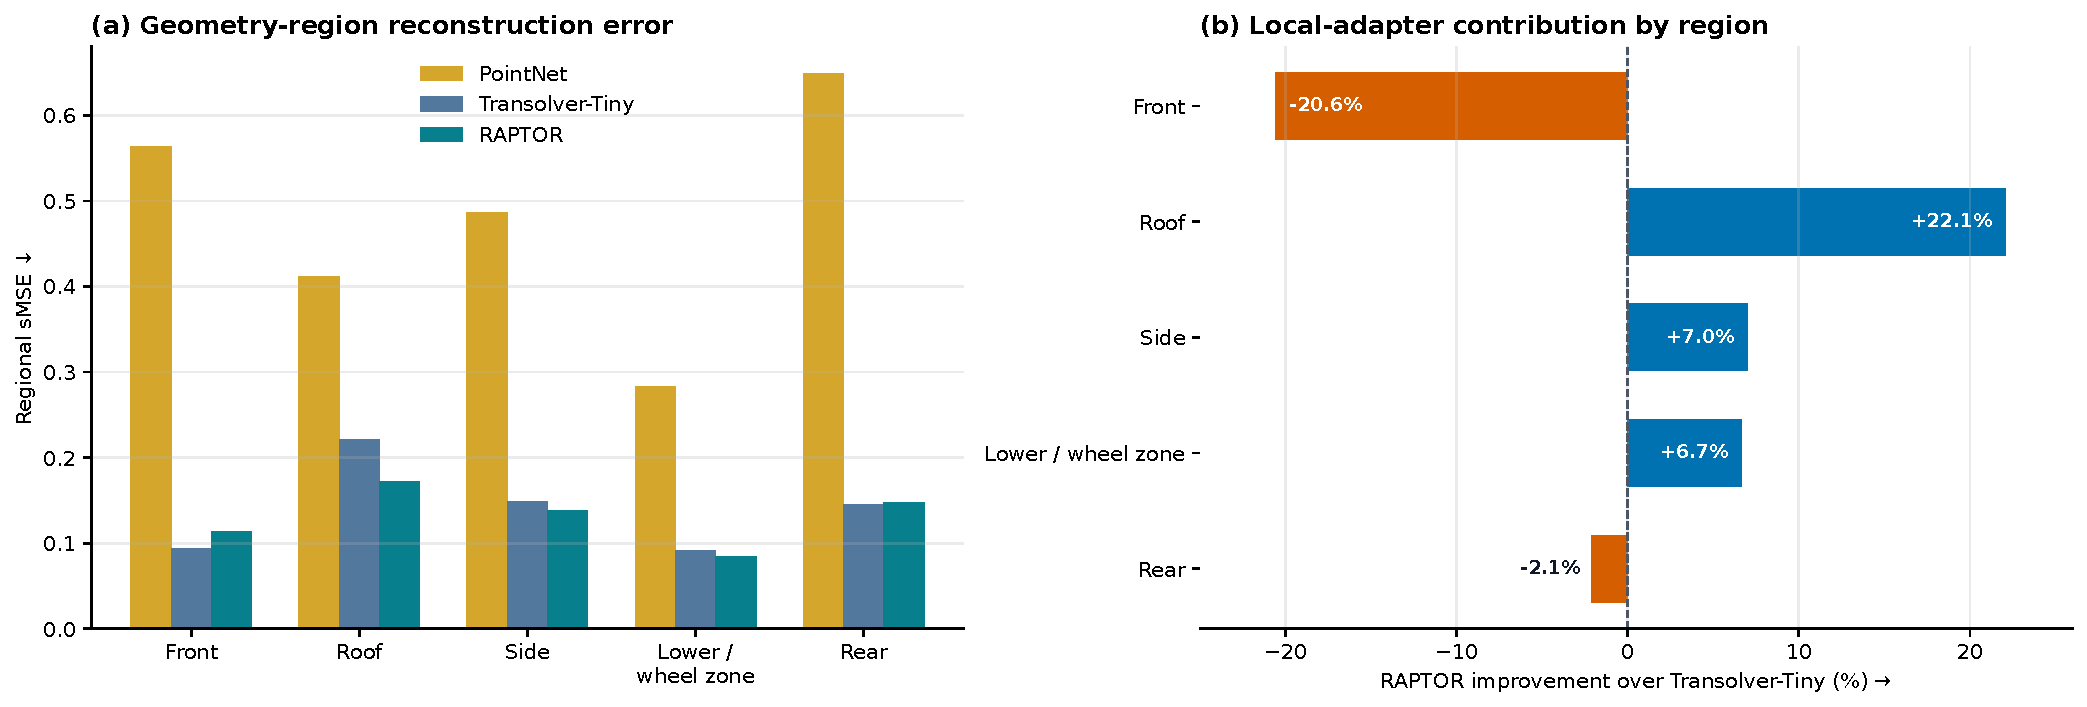
\includegraphics[
		width=\linewidth,
		keepaspectratio
		]{figs/Fig4.pdf}
		\captionof{figure}{Region-wise reconstruction errors and local-adapter contributions
			on the ten-vehicle test set from the 100-vehicle experiment. (a) Mean sMSEs of PointNet,
			Transolver-Tiny, and RAPTOR over five vehicle-relative surface regions.
			(b) Relative regional improvement of RAPTOR over Transolver-Tiny.
			Positive values indicate lower errors for RAPTOR, whereas negative values
			indicate regional degradation. The local adapter provides the largest
			improvement over the roof, followed by the side and lower/wheel zone, but
			does not improve the front and rear regions.}
		\label{fig4}
	\end{minipage}
\end{center}

Relative to Transolver-Tiny, RAPTOR lowers the mean regional error by
22.1\% on the roof, 7.0\% on the side, and 6.7\% in the lower/wheel
region. In contrast, its errors increase by 20.6\% at the front and 2.1\%
at the rear. The local adapter is therefore most effective over the roof,
side, and lower-body regions in the current experiment, but it does not
uniformly improve every geometric region.

This observation is consistent with the per-vehicle comparison. The largest
individual gain is 28.64\%, whereas the identified regression case exhibits
a 9.51\% increase in error. The overall improvement consequently reflects a
majority trend rather than universal dominance on every geometry.

RAPTOR increases the parameter count by 25.7\% and peak allocated memory by
13.5\%. The elapsed times in Table~\ref{tab:automobile_results} come from
independent single runs and are reported descriptively; without repeated
timing measurements and variability estimates, they do not isolate
architecture-only overhead.

\FloatBarrier
\subsection{Evaluation on three-dimensional aircraft geometries}
\label{subsec:aircraft_results}

The aircraft experiment evaluates the same RAPTOR architecture on four
three-dimensional aircraft families. Both models are trained from scratch
on the aircraft split. Table~\ref{tab:aircraft_overall} reports the results.

\begin{table}[H]
    \centering
    \caption{Overall results for the 100-aircraft geometry experiment.}
    \label{tab:aircraft_overall}
    \renewcommand{\arraystretch}{1.10}
    \setlength{\tabcolsep}{5pt}
    \begin{tabular}{lrrrrr}
        \toprule
        Model
        & Test sMSE
        & Best val. sMSE
        & Parameters
        & Memory
        & Time \\
        &
        &
        & 
        & (MiB)
        & (s) \\
        \midrule
        Transolver-Tiny
        & 0.843596 & 0.5532 & 195,345 & 103.76 & 1795.3 \\
        RAPTOR
        & \textbf{0.771331} & \textbf{0.4954}
        & 245,525 & 117.77 & 1929.6 \\
        \bottomrule
    \end{tabular}
\end{table}

RAPTOR reduces the overall test sMSE by 8.57\% and the best validation sMSE
by 10.45\% relative to Transolver-Tiny. It also completes early stopping
after 91 epochs, compared with 96 epochs for the baseline. The total training
time nevertheless increases by approximately 7.5\%, reflecting the
additional cost of neighborhood aggregation.

\begin{center}
	\begin{minipage}{0.94\linewidth}
		\centering
		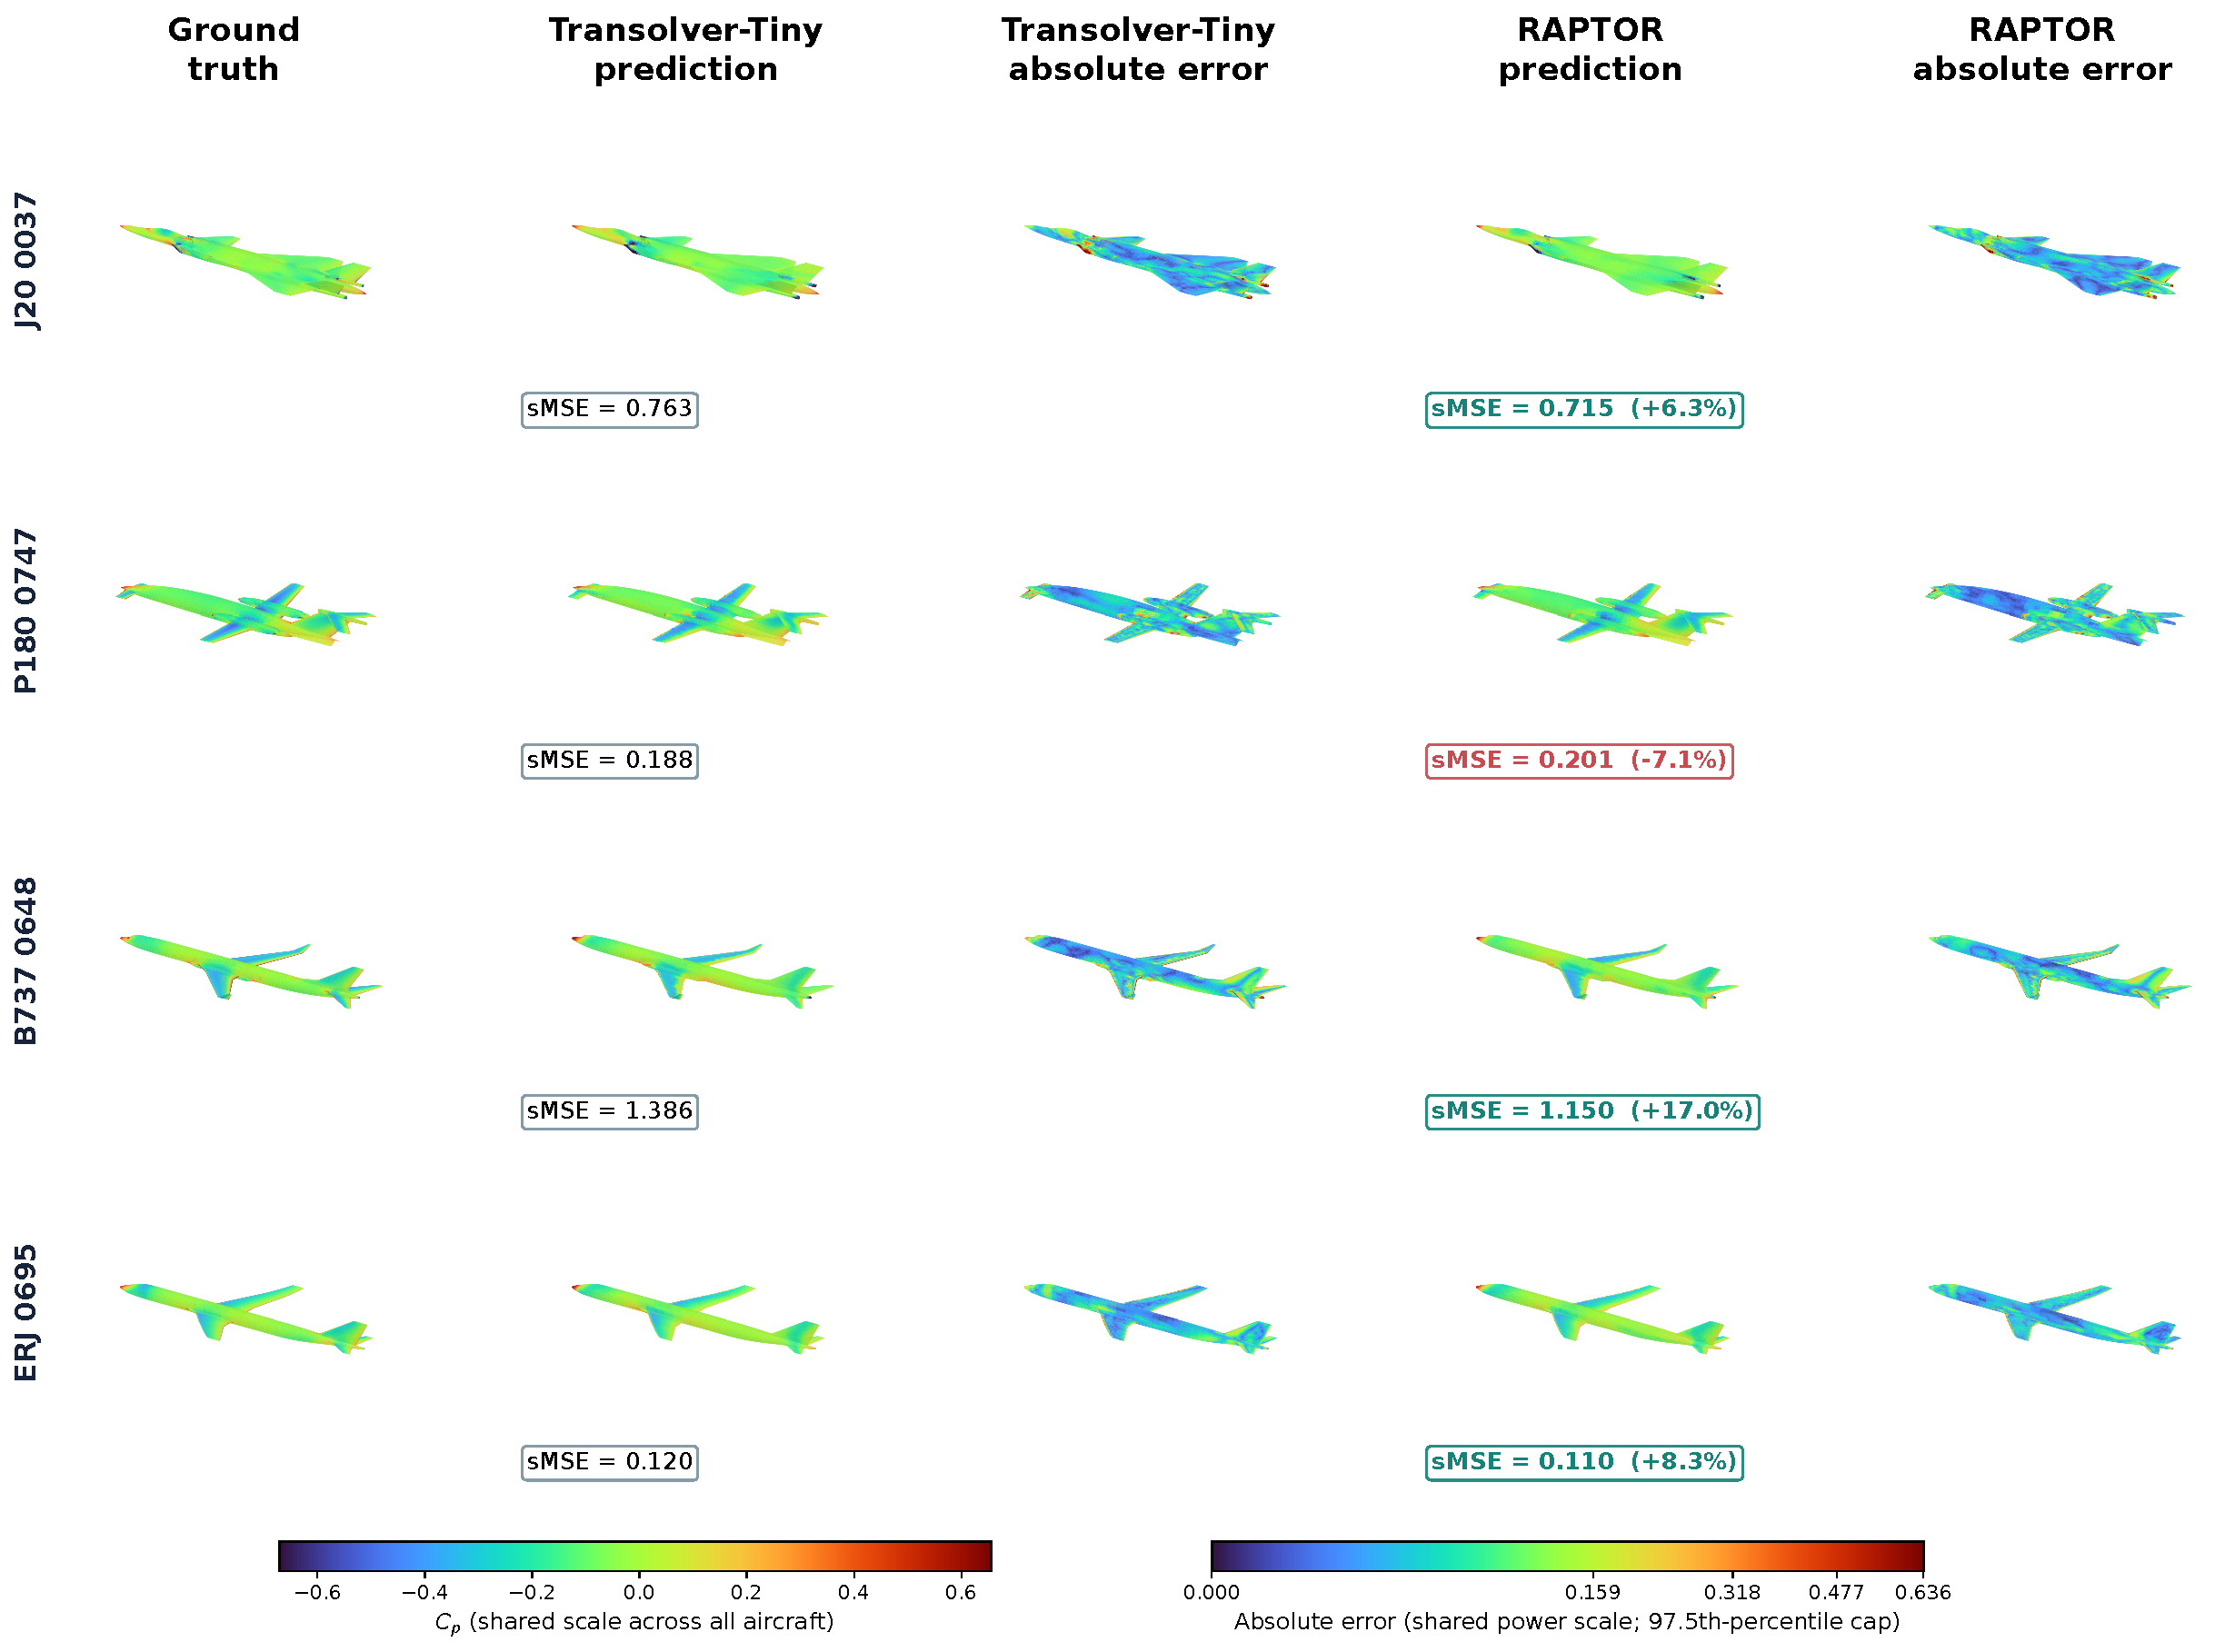
\includegraphics[
		width=\linewidth,
		keepaspectratio
		]{figs/Fig5.pdf}
		\captionof{figure}{Representative aircraft \(C_p\) reconstruction for
			J20 sample 0037, P180 sample 0747, Boeing 737 sample 0648, and ERJ
			sample 0695. Columns show ground truth, Transolver-Tiny prediction and
			absolute error, and RAPTOR prediction and absolute error. Predictions
			and ground truth share a common field scale across the figure; all error
			maps use a common power-normalized error scale.}
		\label{fig5}
	\end{minipage}
\end{center}

Figure~\ref{fig5} compares representative samples from
the four aircraft families. RAPTOR reproduces the principal spatial
variation of \(C_p\) across configurations with substantially different
wings, fuselages, and tail structures. The residual-error maps are
spatially nonuniform and tend to concentrate near geometrically intricate
or rapidly varying regions.

The family-level statistics in Table~\ref{tab:aircraft_family} and
Figure~\ref{fig5} reveal that the overall 8.57\%
improvement is not distributed equally among the four aircraft types.




RAPTOR improves the mean error for J20, Boeing 737, and ERJ, but performs
8.46\% worse for P180. It wins on six of the ten individual aircraft and
loses on four. This fixed-split result shows that RAPTOR can be applied to aircraft
surface geometries without changing its principal architecture. At the same
time, it identifies an important applicability boundary: a fixed
12-nearest-neighbor correction is not equally beneficial for every tested
geometry. With only two P180 test objects, the result cannot be attributed to
the family as a whole; it instead motivates further investigation of adaptive
neighborhood scale, sampling density, and gate behavior.

\begin{center}
    \begin{minipage}{0.82\linewidth}
        \centering
        \captionof{table}{Aircraft-family test sMSE and RAPTOR improvement over
    Transolver-Tiny.}
    \label{tab:aircraft_family}
    \renewcommand{\arraystretch}{1.10}
    \setlength{\tabcolsep}{4.5pt}
    \begin{tabular}{lrrrr}
        \toprule
        Family
        & Test samples
        & Transolver
        & RAPTOR
        & Improvement \\
        \midrule
        J20
        & 2 & 0.687817 & \textbf{0.661924} & \(+3.76\%\) \\
        P180
        & 2 & \textbf{0.182439} & 0.197882 & \(-8.46\%\) \\
        Boeing 737
        & 3 & 2.114592 & \textbf{1.888884} & \(+10.67\%\) \\
        ERJ
        & 3 & 0.117223 & \textbf{0.109015} & \(+7.00\%\) \\
        \bottomrule
    \end{tabular}
    \end{minipage}
\end{center}

Figure~\ref{fig6} presents the best paired case selected from the
complete held-out aircraft test set according to the relative
sMSE improvement of RAPTOR over Transolver-Tiny. For Boeing
737 sample 0483, RAPTOR reduces the sMSE from 3.26323 to 2.69088,
corresponding to an improvement of 17.54\%. Compared with the
Transolver-Tiny error map, the RAPTOR result exhibits smaller deviations
over several geometrically sensitive regions, particularly the wing
surfaces, wing--body junctions, and tail assembly. This spatial pattern
is consistent with the intended role of the local adapter in recovering
neighborhood-scale information that may be weakened during
physics-token compression.

\begin{center}
	\begin{minipage}{0.98\linewidth}
		\centering
		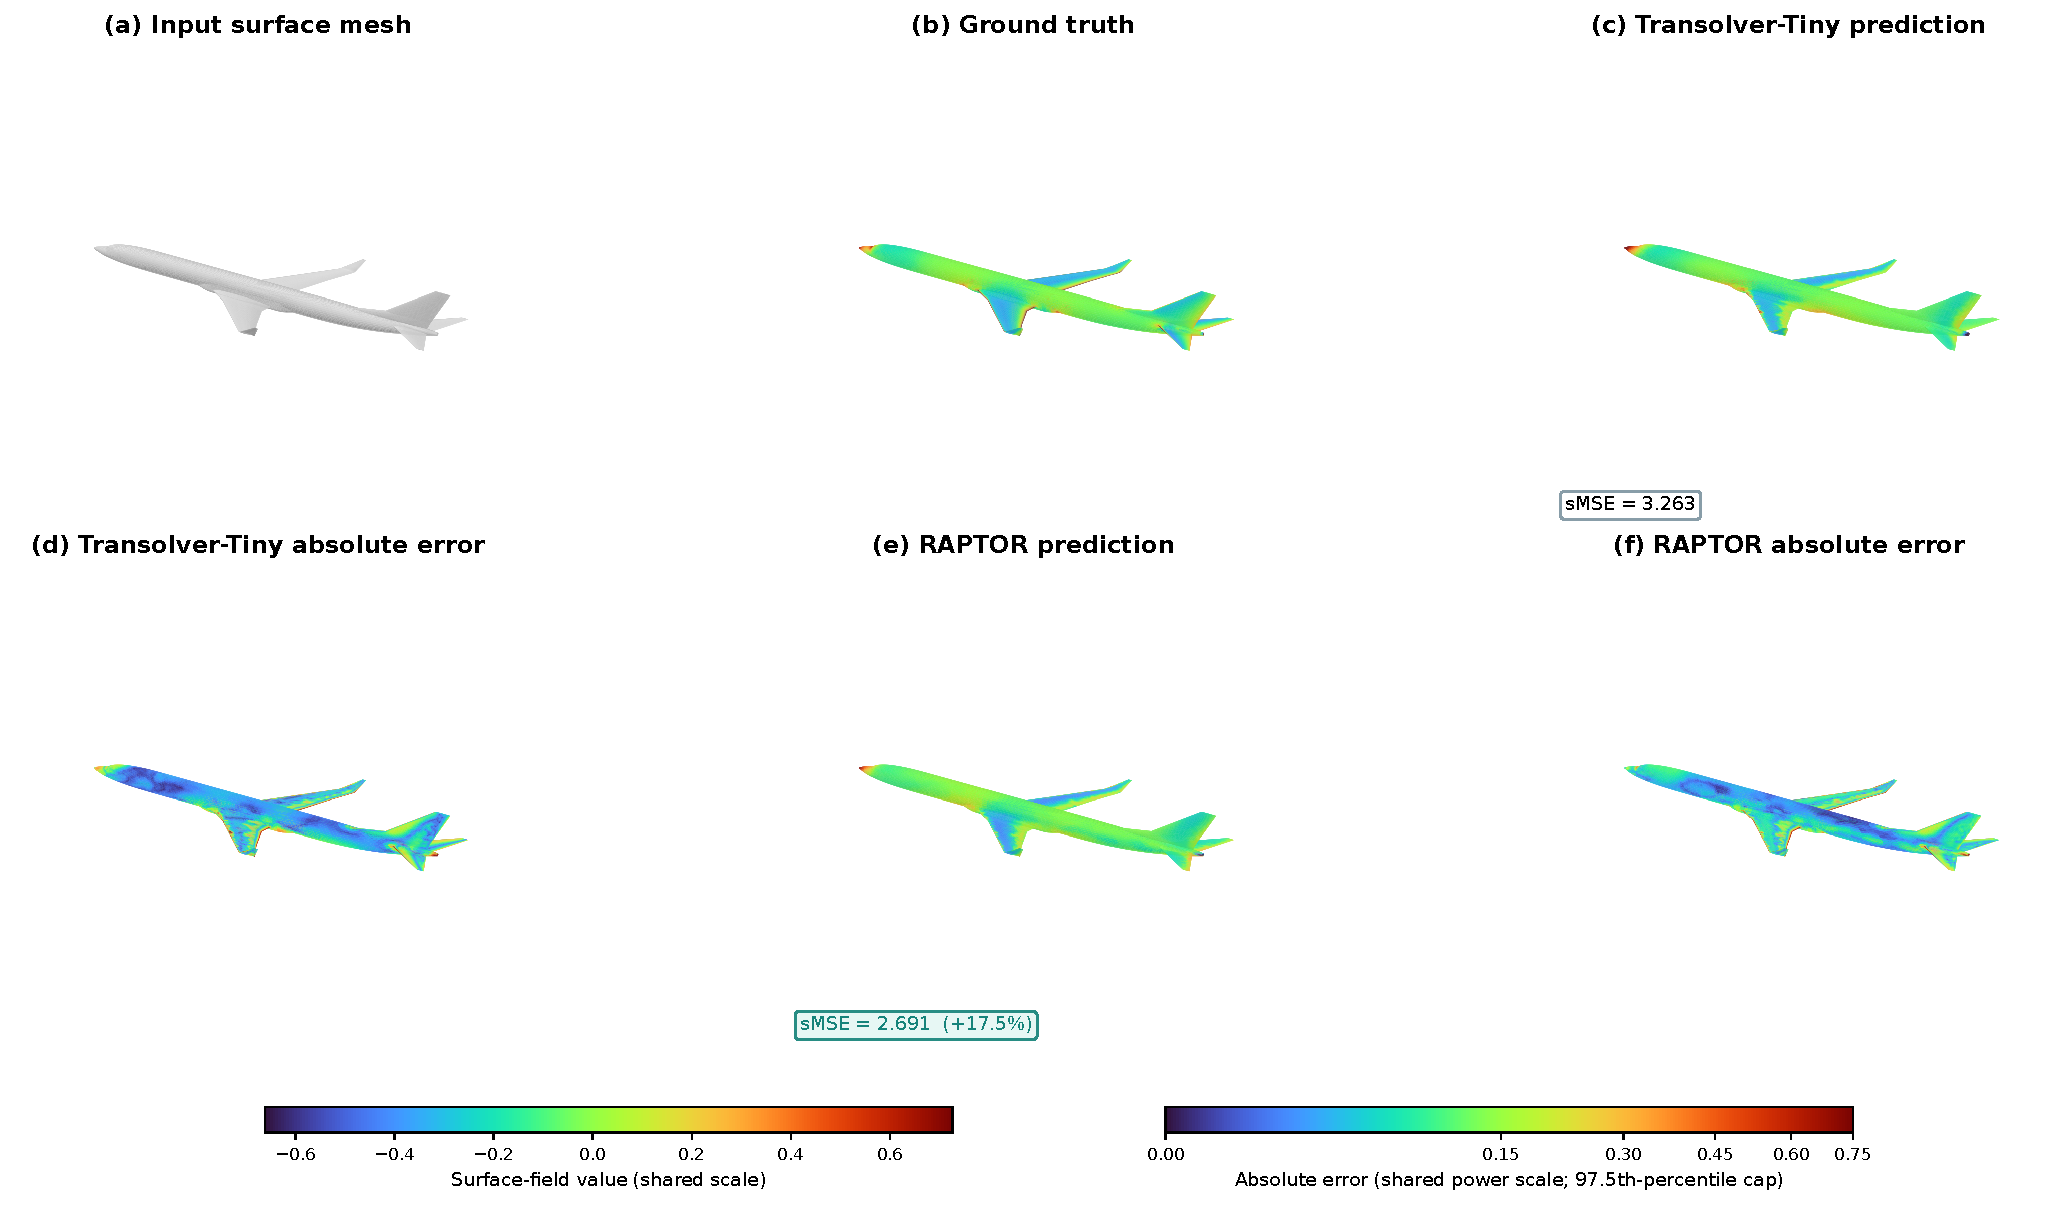
\includegraphics[
		width=\linewidth,
		keepaspectratio
		]{figs/fig6.pdf}
		\captionof{figure}{
			Best paired aircraft \(C_p\)-reconstruction case in
			the complete held-out test set. For Boeing 737 sample 0483,
			RAPTOR reduces the sMSE from 3.26323 to 2.69088,
			corresponding to a relative improvement of 17.54\% over
			Transolver-Tiny. Panels (a)--(f) show the input surface
			mesh, ground truth, Transolver-Tiny prediction,
			Transolver-Tiny absolute error, RAPTOR prediction, and
			RAPTOR absolute error, respectively. The ground truth and
			predictions share a common field scale, while the two
			absolute-error maps share a common error scale.
		}
		\label{fig6}
	\end{minipage}
\end{center}

Figure~\ref{fig7} presents the worst paired case in the same held-out
test set. For P180 sample 1118, the sMSE increases from 0.17730
for Transolver-Tiny to 0.19492 for RAPTOR, corresponding to a relative
improvement of $-9.94\%$. Although both models preserve the overall
\(C_p\) distribution, the RAPTOR error map indicates that the
local correction does not reduce the remaining error for this geometry
and slightly increases deviations over parts of the wing surfaces and
component-junction regions.

\begin{center}
	\begin{minipage}{0.98\linewidth}
		\centering
		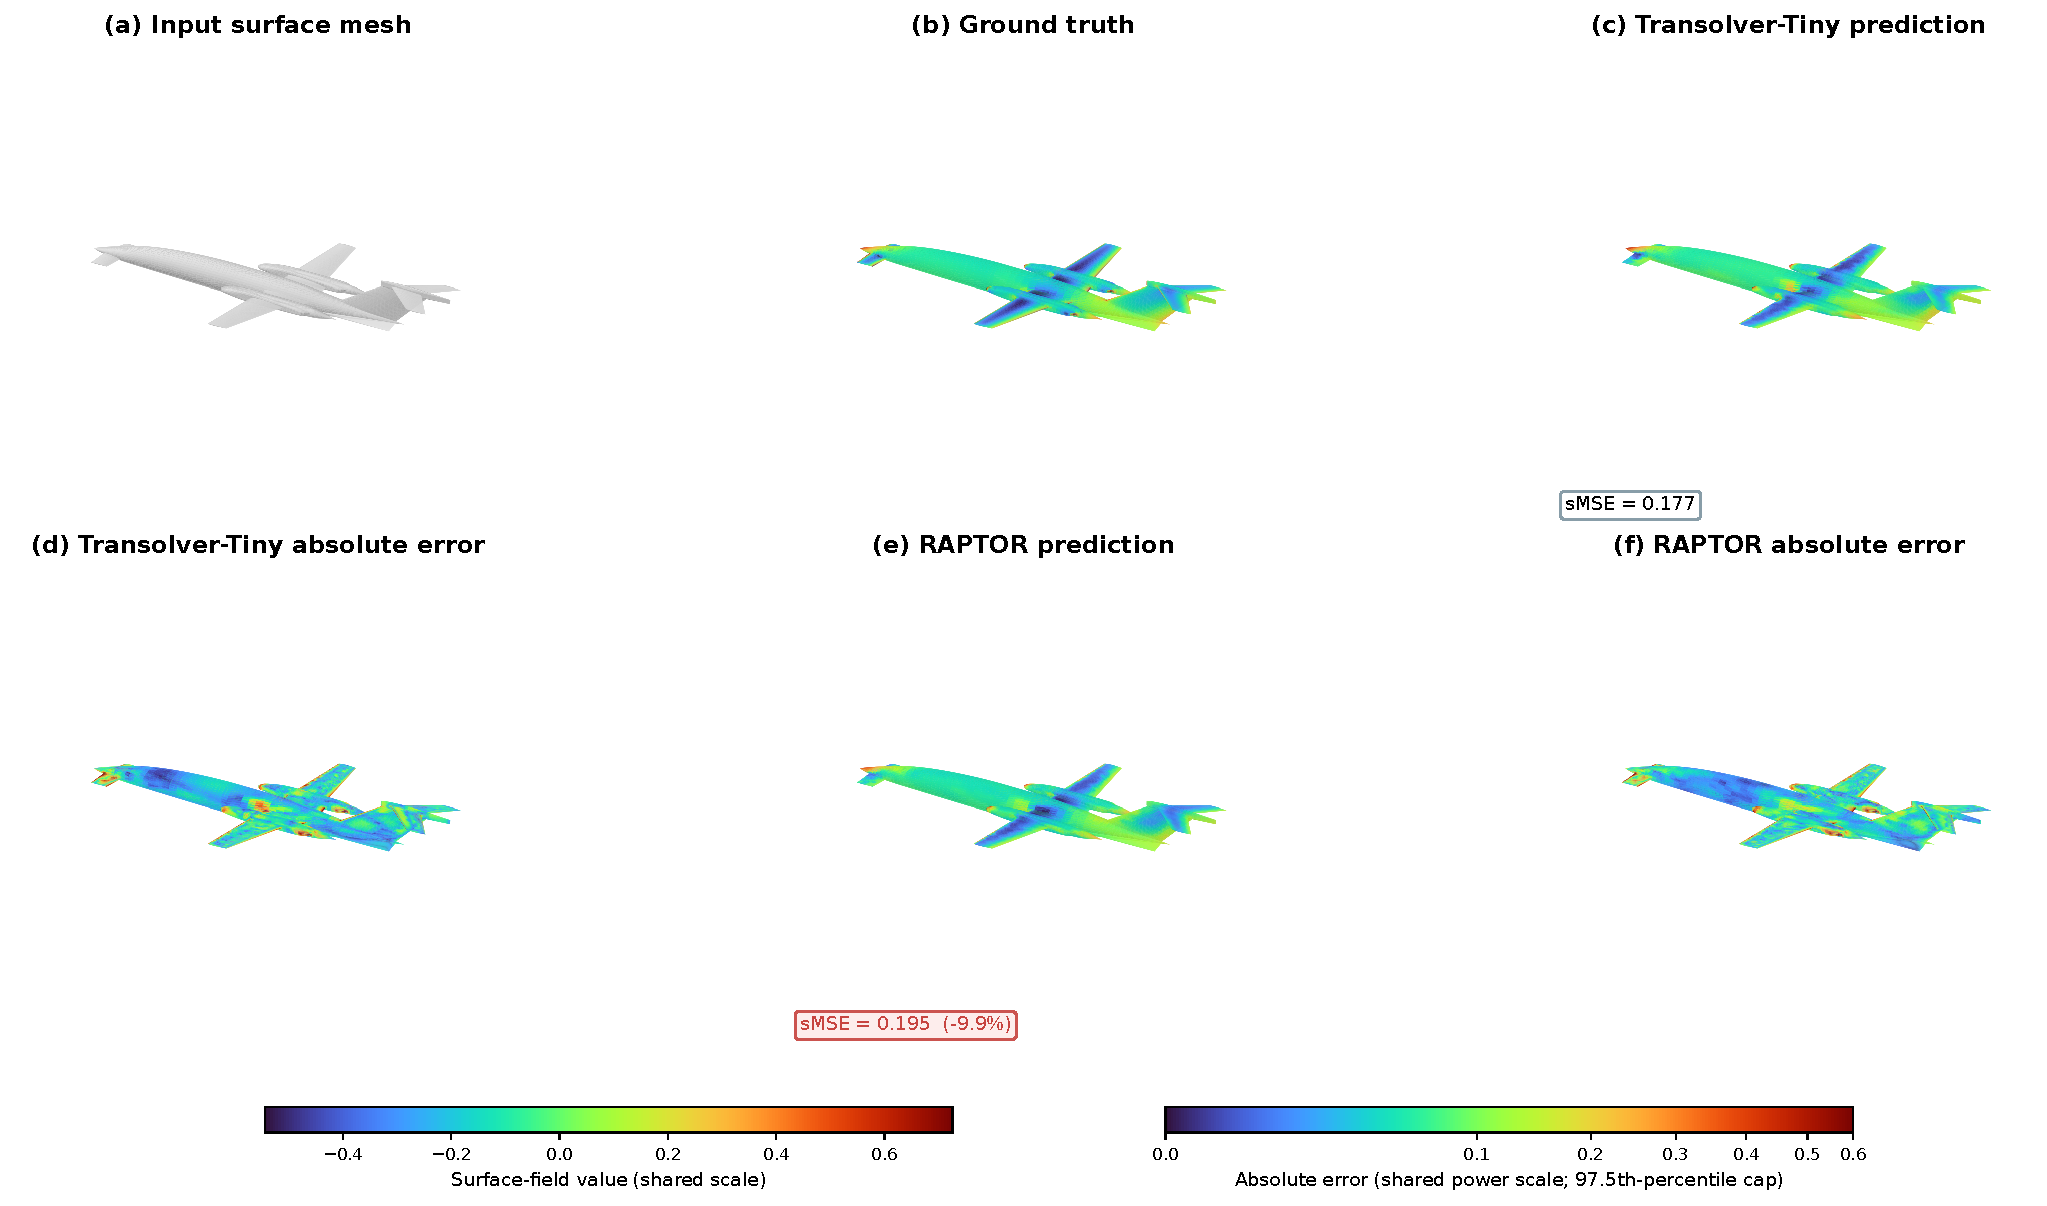
\includegraphics[
		width=\linewidth,
		keepaspectratio
		]{figs/fig7.pdf}
		\captionof{figure}{
			Worst paired aircraft \(C_p\)-reconstruction case in
			the complete held-out test set. For P180 sample 1118, the
			sMSE increases from 0.17730 for Transolver-Tiny to
			0.19492 for RAPTOR, corresponding to a relative improvement
			of $-9.94\%$. Panels (a)--(f) show the input surface mesh,
			ground truth, Transolver-Tiny prediction,
			Transolver-Tiny absolute error, RAPTOR prediction, and
			RAPTOR absolute error, respectively. The ground truth and
			predictions share a common field scale, while the two
			absolute-error maps share a common error scale.
		}
		\label{fig7}
	\end{minipage}
\end{center}

Taken together, these two cases show that residual local adaptation is
not uniformly beneficial for every aircraft geometry. RAPTOR's overall
advantage should therefore be interpreted as an average improvement under
the present fixed split and seed, rather than a universal per-sample gain.
In both figures, the full-surface colors are used only for
visualization and are obtained by interpolating the predictions from
the matched 4,096 sampled nodes onto the original aircraft surface
mesh. All reported sMSE values are computed directly on the
matched sampled nodes rather than on the interpolated full-surface
fields.

\subsection{Empirical node-scaling and resource profile}
\label{subsec:node_scaling}

Figure~\ref{fig:node_scaling} and Table~\ref{tab:node_scaling} report the
isolated node-scaling profile under the fixed configuration
\(S=64\), \(K=12\), \(d=64\), \(L=4\), and \(H=4\). Latency markers and
error bars represent the mean and one sample standard deviation over
30 timed iterations for the model measurements. Transolver-Tiny and
RAPTOR complete both forward and full mixed-precision training steps at
\(N=16384\). At that resolution, their mean training-step latencies are
\(49.37\pm2.33\)~ms and \(66.99\pm1.07\)~ms, respectively, while their
peak allocated GPU memories are 350.70~MiB and 410.31~MiB. From
\(N=4096\) to \(N=16384\), the corresponding memory footprints increase
by factors of 3.41 and 3.50 for a fourfold increase in node count.

RAPTOR's mean training-step latency is not strictly monotonic at the
intermediate node counts: it changes from \(54.18\pm6.27\)~ms at
\(N=2048\) to \(42.77\pm8.09\)~ms at \(N=4096\) and
\(44.40\pm4.15\)~ms at \(N=8192\). The overlapping
one-standard-deviation ranges indicate that these intermediate
differences should not be interpreted as an algorithmic speedup with
increasing \(N\). They are consistent with timing variability and
changes in kernel-launch overhead and GPU utilization. The overall
memory trend remains consistent with the linear-in-\(N\) activation
structure expected when \(S\), \(K\), \(d\), and \(L\) are fixed.

The explicit dense-attention baseline exhibits a different scaling
regime. Its training-step allocation increases from 154.91~MiB at
\(N=1024\) to 2098.40~MiB at \(N=4096\). At \(N=8192\), the training
step completes only through Windows Display Driver Model shared-memory
spillover: its peak CUDA allocation reaches 8274.59~MiB, exceeding the
6141~MiB physical device memory, and its mean latency reaches
\(12.51\pm0.35\)~s. \mbox{Dense attention at \(N=16384\) was not attempted
to avoid further memory oversubscription.} Accordingly, the
\(N=8192\) result should be interpreted as a spillover measurement
rather than a conventional in-device-memory result.

\begin{center}
    \begin{minipage}{\linewidth}
        \centering
    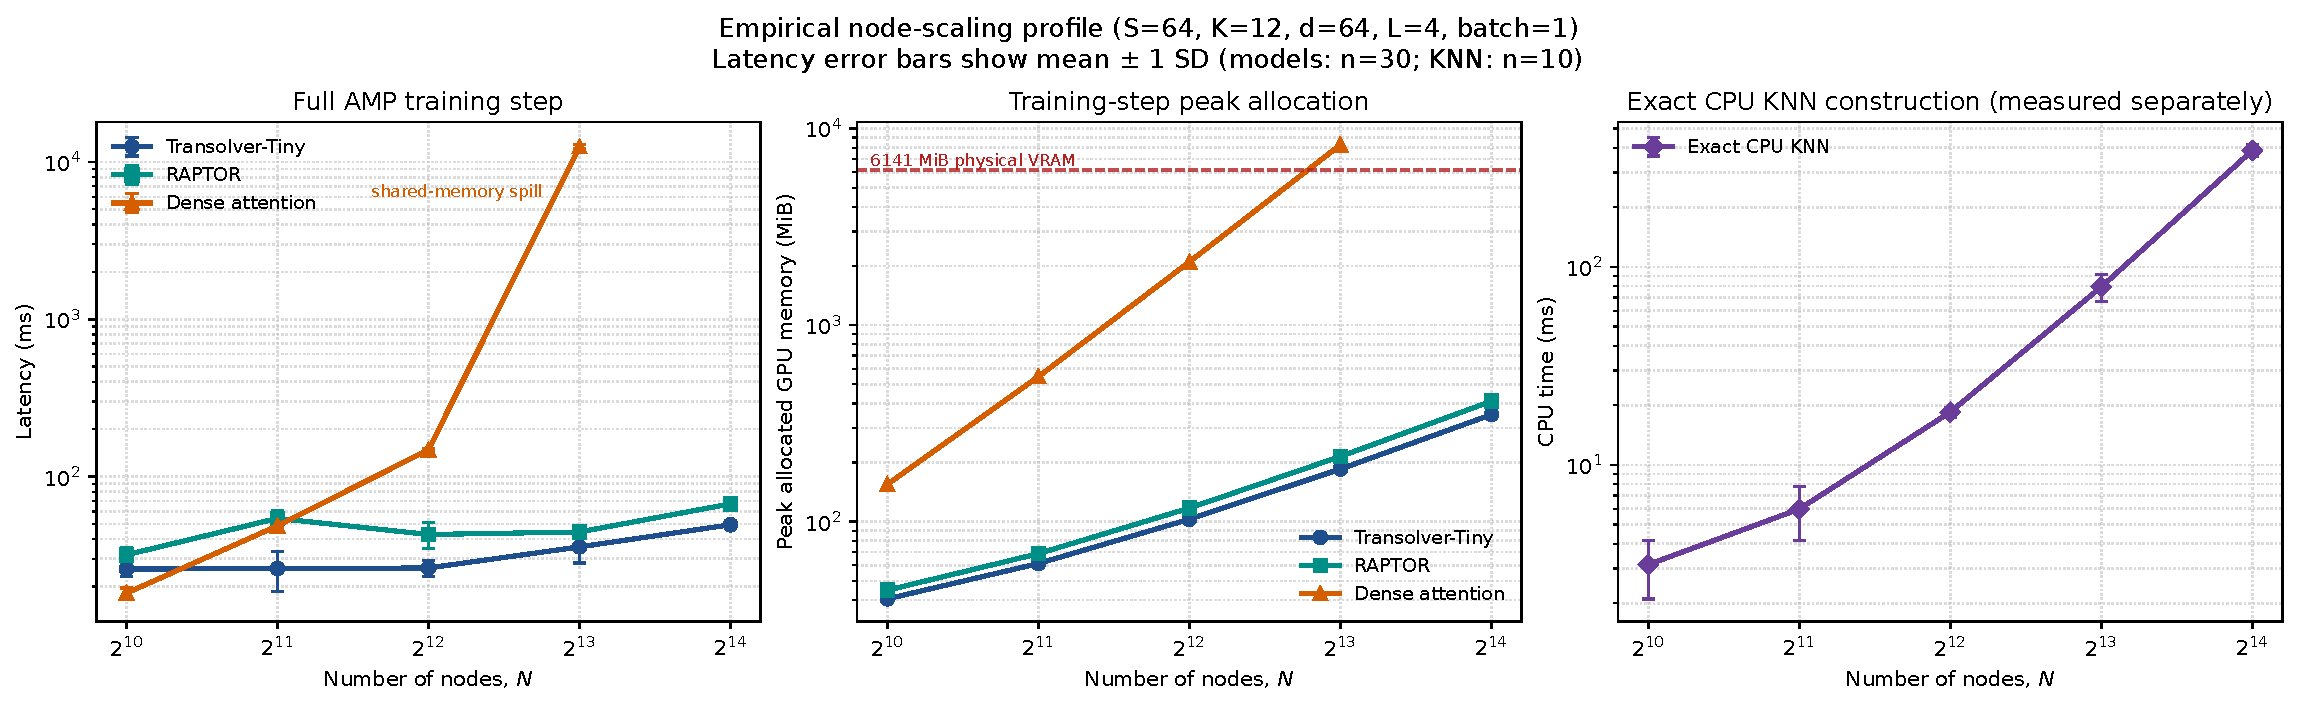
\includegraphics[width=\linewidth,keepaspectratio]{figs/fig8_node_scaling.pdf}
   \captionof{figure}{Empirical node-scaling profile on the RTX 4050 Laptop GPU.
   	The left panel reports the mean latency of a complete CUDA-AMP AdamW
   	training step, with error bars denoting one sample standard deviation
   	over 30 timed iterations. The center panel reports peak allocated
   	training-step GPU memory; error bars are not applicable because this
   	quantity is the maximum allocation observed during each measured
   	phase. The right panel reports the separately measured exact CPU
   	\(K\)-NN construction time, with error bars denoting one sample
   	standard deviation over 10 timed runs. Transolver-Tiny and RAPTOR use
   	physics-token interaction with \(S=64\); RAPTOR additionally uses
   	precomputed \(K=12\) neighbor indices. The dense baseline explicitly
   	materializes per-head \(N\times N\) attention scores. Its
   	\(N=8192\) training step allocates 8274.59~MiB, exceeding the
   	6141~MiB physical GPU memory and invoking shared-memory spillover.
   	Dense attention at \(N=16384\) was not attempted to avoid further
   	memory oversubscription.}
    \label{fig:node_scaling}
    \end{minipage}
\end{center}

\begin{center}
    \begin{minipage}{1.00\linewidth}
        \centering
        \captionof{table}{Measured node-scaling results. Each model entry reports
		forward latency/training-step latency/peak allocated training-step
		memory in ms/ms/MiB. Model latencies are means over 30 timed
		iterations, whereas memory values are peak allocations. The \(K\)-NN
		column reports mean construction time \(\pm\) one sample standard
		deviation over 10 timed runs. The final column gives the memory
		required to materialize the FP32 pairwise-distance matrix.}
	\label{tab:node_scaling}
	\renewcommand{\arraystretch}{1.12}
	\setlength{\tabcolsep}{3.5pt}
	\scriptsize
	\resizebox{\linewidth}{!}{%
		\begin{tabular}{rccccc}
			\toprule
			\(N\)
			& Transolver-Tiny
			& RAPTOR
			& Dense attention
			& \shortstack{KNN construction\\(mean \(\pm\) SD, ms)}
			& \shortstack{KNN distance\\matrix (MiB)} \\
			\midrule
			1024
			& 6.34/25.80/40.50
			& 9.25/31.76/44.82
			& 5.10/18.13/154.91
			& \(3.14\pm1.03\) 
			& 4 \\
			
			2048
			& 6.30/25.95/61.27
			& 14.31/54.18/68.79
			& 19.08/48.58/546.74
			& \(5.98\pm1.82\) 
			& 16 \\
			
			4096
			& 6.58/26.21/102.94
			& 14.27/42.77/117.33
			& 53.07/147.83/2098.40
			& \(18.47\pm1.04\)
			& 64 \\
			
			8192
			& 8.91/35.67/185.29
			& 13.53/44.40/214.75
			& 181.95/12512.48/8274.59\(^{\dagger}\)
			& \(79.21\pm12.50\)
			& 256 \\
			
			16384
			& 14.31/49.37/350.70
			& 21.74/66.99/410.31
			& --
			& \(386.52\pm26.99\)
			& 1024 \\
			\bottomrule
		\end{tabular}%
	}
	\vspace{2pt}
	
	\begin{minipage}{0.98\linewidth}
		\footnotesize
		The distance-matrix footprint is calculated as
		\(4N^2/2^{20}\) MiB for an FP32 \(N\times N\) matrix.
		\(^{\dagger}\)The dense-attention run completed using WDDM
		shared-memory spillover; its allocation exceeds the
		6141~MiB physical GPU capacity and therefore is not an
		in-device-memory result. Dense attention at \(N=16{,}384\) was not attempted to avoid further memory oversubscription.
	\end{minipage}
    \end{minipage}
\end{center}

Exact Euclidean \(K\)-NN construction remains separate from the model
measurements. Based on 10 timed runs at each node count, its mean CPU
construction time increases from \(3.14\pm1.03\)~ms at \(N=1024\) to
\(386.52\pm26.99\)~ms at \(N=16384\). Meanwhile, the materialized FP32
pairwise-distance matrix grows from 4~MiB to 1024~MiB. Its memory
footprint increases by a factor of four whenever \(N\) doubles,
directly reflecting the quadratic \(\mathcal{O}(N^2)\) memory cost of
the exact \texttt{torch.cdist}-based graph-construction procedure.





\section{Conclusions and Future Work}
\label{sec:conclusion}

This study introduced RAPTOR, a neural operator that augments a
Physics-Attention backbone with an explicit node-space \(K\)-NN residual
adapter. The architecture combines token-mediated global communication with
sparse local correction while retaining the computational advantages of
physics-token compression. A bounded, zero-initialized gate ensures that each
RAPTOR block initially reproduces the corresponding Physics-Attention
backbone and allows the local contribution to be introduced progressively
during optimization. Structurally, the resulting operator combines a
per-head conditional node-mixing pathway whose frozen rank is bounded by the
number of physics slices with an \(\mathcal{O}(NK)\) set of direct local
dependencies. This characterization concerns the frozen node-mixing pattern
and should not be interpreted as a rank bound on the complete nonlinear
operator or its Jacobian.

Under the reported fixed splits and single training seed, RAPTOR achieved the
lowest macro error among the evaluated models on both AirfRANS extrapolation
tasks. Its macro relative \(L_2\) errors were \(0.2219\) for Reynolds-number
extrapolation and \(0.2969\) for angle-of-attack extrapolation. The ablation
results further indicate that the local adapter improves the matched
Physics-Attention backbone on the AoA task and that zero initialization is
preferable to introducing a nonzero local correction at the start of
training. These observations support the intended baseline-preserving role
of the gate, although they do not constitute a general optimization or
convergence guarantee.

The three-dimensional experiments provide additional evidence that the
global and local pathways are complementary. Relative to Transolver-Tiny,
RAPTOR reduced the automobile test sMSE from \(0.145534\) to \(0.135684\),
corresponding to a \(6.77\%\) improvement, and reduced the aircraft test sMSE
by \(8.57\%\). Nevertheless, the object-level results show that the benefit
is not universal: RAPTOR improved seven of ten automobile objects and six of
ten aircraft objects, while several individual geometries exhibited higher
errors. The reported gains should therefore be interpreted as average
improvements under the present protocols rather than guaranteed
per-geometry behavior. Similarly, the measurements at \(N=4096\) demonstrate
feasibility on the specified RTX 4050 laptop GPU. The isolated node-scaling
profile further shows that Transolver-Tiny and RAPTOR complete mixed-precision
training steps at \(N=16384\) with peak allocations of 350.70~MiB and
410.31~MiB, whereas explicit dense attention exceeds physical GPU memory at
\(N=8192\). These measurements provide implementation-level evidence over
the tested range, but they do not establish an accuracy--resource Pareto
advantage or hardware-independent scalability.

Future work should first evaluate multiple training seeds and larger
object-level test sets to separate split-dependent variation from training
randomness. Resource evaluation should next vary \(S\) and \(K\), extend
large-\(N\) measurements to additional hardware, and include end-to-end data
movement, preprocessing, throughput, and accuracy--resource Pareto curves.
The exact pairwise \(K\)-NN construction reaches
\(386.52\pm26.99\)~ms over 10 timed runs and requires a 1024~MiB
distance matrix at \(N=16384\), motivating cached, approximate, or
geometry-aware graph builders for substantially larger meshes. The local
connectivity also warrants further study because Euclidean neighbors can
form nonphysical links across thin wings, vehicle gaps, or nearby but
geodesically distant surfaces. Comparisons with mesh-edge, geodesic,
radius-based, and adaptive neighborhoods may therefore improve both physical
consistency and robustness. Finally, future analyses should quantify the
realized contribution of the local branch through layer-wise norm ratios
such as $\frac{\left\|\gamma_l\mathbf{M}_{\mathrm{loc}}^{(l)}\right\|_F}
{\left\|\mathbf{Z}_{\mathrm{PA}}^{(l)}\right\|_F},$
rather than interpreting the sign or magnitude of the scalar gate alone.
These extensions would clarify when explicit local adaptation is most useful
and whether its benefits persist across resolutions, geometry families, and
hardware regimes.

% Figure



% Numbered list
% Use the style of numbering in square brackets.
% If nothing is used, default style will be taken.
%\begin{enumerate}[a)]
%\item 
%\item 
%\item 
%\end{enumerate}  

% Unnumbered list
%\begin{itemize}
%\item 
%\item 
%\item 
%\end{itemize}  

% Description list
%\begin{description}
%\item[]
%\item[] 
%\item[] 
%\end{description}  

\clearpage %%Remove this from your manuscript






% Uncomment and use as the case may be
%\begin{theorem} 
%\end{theorem}

% Uncomment and use as the case may be
%\begin{lemma} 
%\end{lemma}

%% The Appendices part is started with the command \appendix;
%% appendix sections are then done as normal sections
%% \appendix





%% To print the credit authorship contribution details
%\printcredits
%
%\section*{Declaration of competing interest}
%\par The authors declare that they have no known competing financial interests or personal relationships that could have appeared to influence the work reported in this paper.
%
%
%\section*{Acknowledgment and funding}
%======================
%%Partially supported by the Postgraduate Research Practice Innovation Program of Jiangsu Province, the China Scholarship Council (Grant No. 202406840118), the National Natural Science Foundation of China (No. 12331006), the Strategic Priority Research Program of the Chinese Academy of Sciences (No. XDB0900100), and the National Key Research and Development Program of China (Nos. 2024YFA1013603, 2024YFA1013600).
%
%\section*{Data availability}
%\par Experimental code and results are available on GitHub. \url{https://github.com/XuChengaq/RAHC} 
%%% Loading bibliography style file
%%\bibliographystyle{model1-num-names}
%\bibliographystyle{cas-model2-names}

% Loading bibliography database
\bibliographystyle{elsarticle-harv} 
\setlength{\bibsep}{0pt}
\renewcommand{\bibfont}{\fontsize{8pt}{9pt}\selectfont}
\bibliography{cas-refs}

% Biography
%\bio{}
% Here goes the biography details.
%\endbio

%\bio{pic1}
% Here goes the biography details.
%\endbio

\end{document}
